
%!TEX ROOT = thesis.tex
\chapter{LITERATURE REVIEW}
\label{chapter: 2}

This chapter would cover the literature review part of this project. The first section would elaborate on the datasets evaluated, including the data exploratory analysis of the datasets.  The second and third sections would include a brief introduction to traditional methods semantic segmentation and their limitations respectively. The fourth sections would serve as a literature review of semantic segmentation using Convolutional Neural Networks. The fifth and last section would include the literature review of semantic segmentation using transformers and its advantages.

\section{Satellite Images Datasets}

\FloatBarrier
\begin{landscape}
\begin{table}[]
\begin{tabular}{|c|c|c|c|c|c|c|}
\hline
\textbf{Dataset}                                                      & \textbf{Source}                                                & \textbf{\# Samples} & \textbf{\# Classes} & \textbf{Size (px)} & \textbf{Res (m)} & \textbf{Band}                                      \\ \hline
\begin{tabular}[c]{@{}c@{}}Benin Cashew \\ Plantation\end{tabular}    & Airbus Pléiades                                                & 70                  & 6                   & 1,122x1,186        & 10               & MSI                                                \\ \hline
\begin{tabular}[c]{@{}c@{}}Cloud Cover \\ Detection\end{tabular}      & Sentinel-2                                                     & 22,728              & 2                   & 512x512            & 10               & MSI                                                \\ \hline
\begin{tabular}[c]{@{}c@{}}Kenya Crop \\ Trade\end{tabular}           & Sentinel-2                                                     & 4,688               & 7                   & 3,035x2,016        & 10               & MSI                                                \\ \hline
\begin{tabular}[c]{@{}c@{}}Deep Globe \\ Land Cover\end{tabular}      & \begin{tabular}[c]{@{}c@{}}DigitalGlobe\\  +Vivid\end{tabular} & 803                 & 7                   & 2,448x2,448        & 0.5              & RGB                                                \\ \hline
DFC2022                                                               & Aerial                                                         & 3,981               & 15                  & 2,000x2,000        & 0.5              & RGB                                                \\ \hline
\begin{tabular}[c]{@{}c@{}}ETCI 2021 \\ Flood Prediction\end{tabular} & Sentinel-1                                                     & 66,810              & 2                   & 256x256            & 5–20             & SAR                                                \\ \hline
GID-15                                                               & Gaofen-2                                                       & 150                 & 15                  & 6,800x7,200        & 3                & RGB                                                \\ \hline
LandCover.ai                                                          & Aerial                                                         & 10,674              & 5                   & 512x512            & 0.25–0.5         & RGB                                                \\ \hline
    LoveDA                                                               & Google Earth                                                   & 5,987               & 7                   & 1,024x1,024        & 0.3              & RGB                                                \\ \hline
Potsdam                                                               & Aerial                                                         & 38                  & 6                   & 4,000x4,000        & 0.02             & RGB                                                \\ \hline
Vaihingen                                                             & Aerial                                                         & 33                  & 6                   & 1,281–3,816        & 0.09             & RGB                                                \\ \hline
SEN12MS                                                               & \begin{tabular}[c]{@{}c@{}}Sentinel-1/2, \\ MODIS\end{tabular} & 180,662             & 33                  & 256x256            & 10               & \begin{tabular}[c]{@{}c@{}}SAR,\\ MSI\end{tabular} \\ \hline
\end{tabular}
\caption{Datasets Reviewed for Semantic Segmentation Task}
\label{tab:datasets}
\end{table}
\end{landscape}

\FloatBarrier

Table \ref{tab:datasets} shows the list of dataset that were evaluated and considered for this project. Each of the dataset is made for semantic segmentation task meaning that each pixel in the dataset is labelled. All of the datasets except for Potsdam and Vaihingen can be downloaded using the TorchGeo library. 

%%Potsdam%%%
The Potsdam and Vaihingen datasets \cite{potsdam-vaihingen} are datasets made specifically for urban semantic segmentation used in the 2D Semantic Labeling Contest - Potsdam and 2D Semantic Labeling Contest - Vaihingen respectively. Both of the datasets are available upon request \href{https://www.isprs.org/education/benchmarks/UrbanSemLab/detection-and-reconstruction.aspx#VaihigenDataDescr}{here}. Although the images are not taken by satellites, a lot of literature reviewed such as \cite{unetformer}, \cite{a-novel-transformer}, \cite{multi-attention-network} and \cite{A2-FPN} train their semantic segmentation model using these datasets thus we think these merit a bit of discussions. Vaihingen dataset is composed of 33 orthorectified image tiles acquired by a near NIR-RGB drone camera, over the town of Vaihingen, Germany. The average size of the images is 20494 x 20064 pixels with a spatial resolution of 9 cm. Potsdam dataset is composed of 38 orthorectified image tiles acquired  over the town of Potsdam using the same NIR-RGB drone camera.. The average size of the tiles is also 20494 x 20064 pixels but with a smaller spatial resolution of 5 cm. Images in both datasets are accompanied by a digital surface model (DSM) representing the absolute height of pixels. There are a total of 6 classes in each dataset: impervious surfaces (roads, concrete surfaces), buildings, low vegetations, trees, cars and clutters (represents uncategorizable land covers).  Figure \ref{fig:potsdam-image} and \ref{fig:potsdam-mask} shows a pair of an image and its corresponding mask from the Potsdam dataset while Figure \ref{fig:vaihingen-image} and \ref{fig:vaihingen-mask} show the ones from Vaihingen dataset.


\begin{figure}[!htb]
    \centering
    \begin{minipage}{0.5\textwidth}
        \centering
        \includegraphics[width=0.95\textwidth, height=0.35\textheight]{images/potsdam-image.png}
        \caption{An Image From Potsdam Dataset \protect\cite{potsdam-vaihingen}}
        \label{fig:potsdam-image}
    \end{minipage}\hfill
    \begin{minipage}{0.5\textwidth}
        \centering
        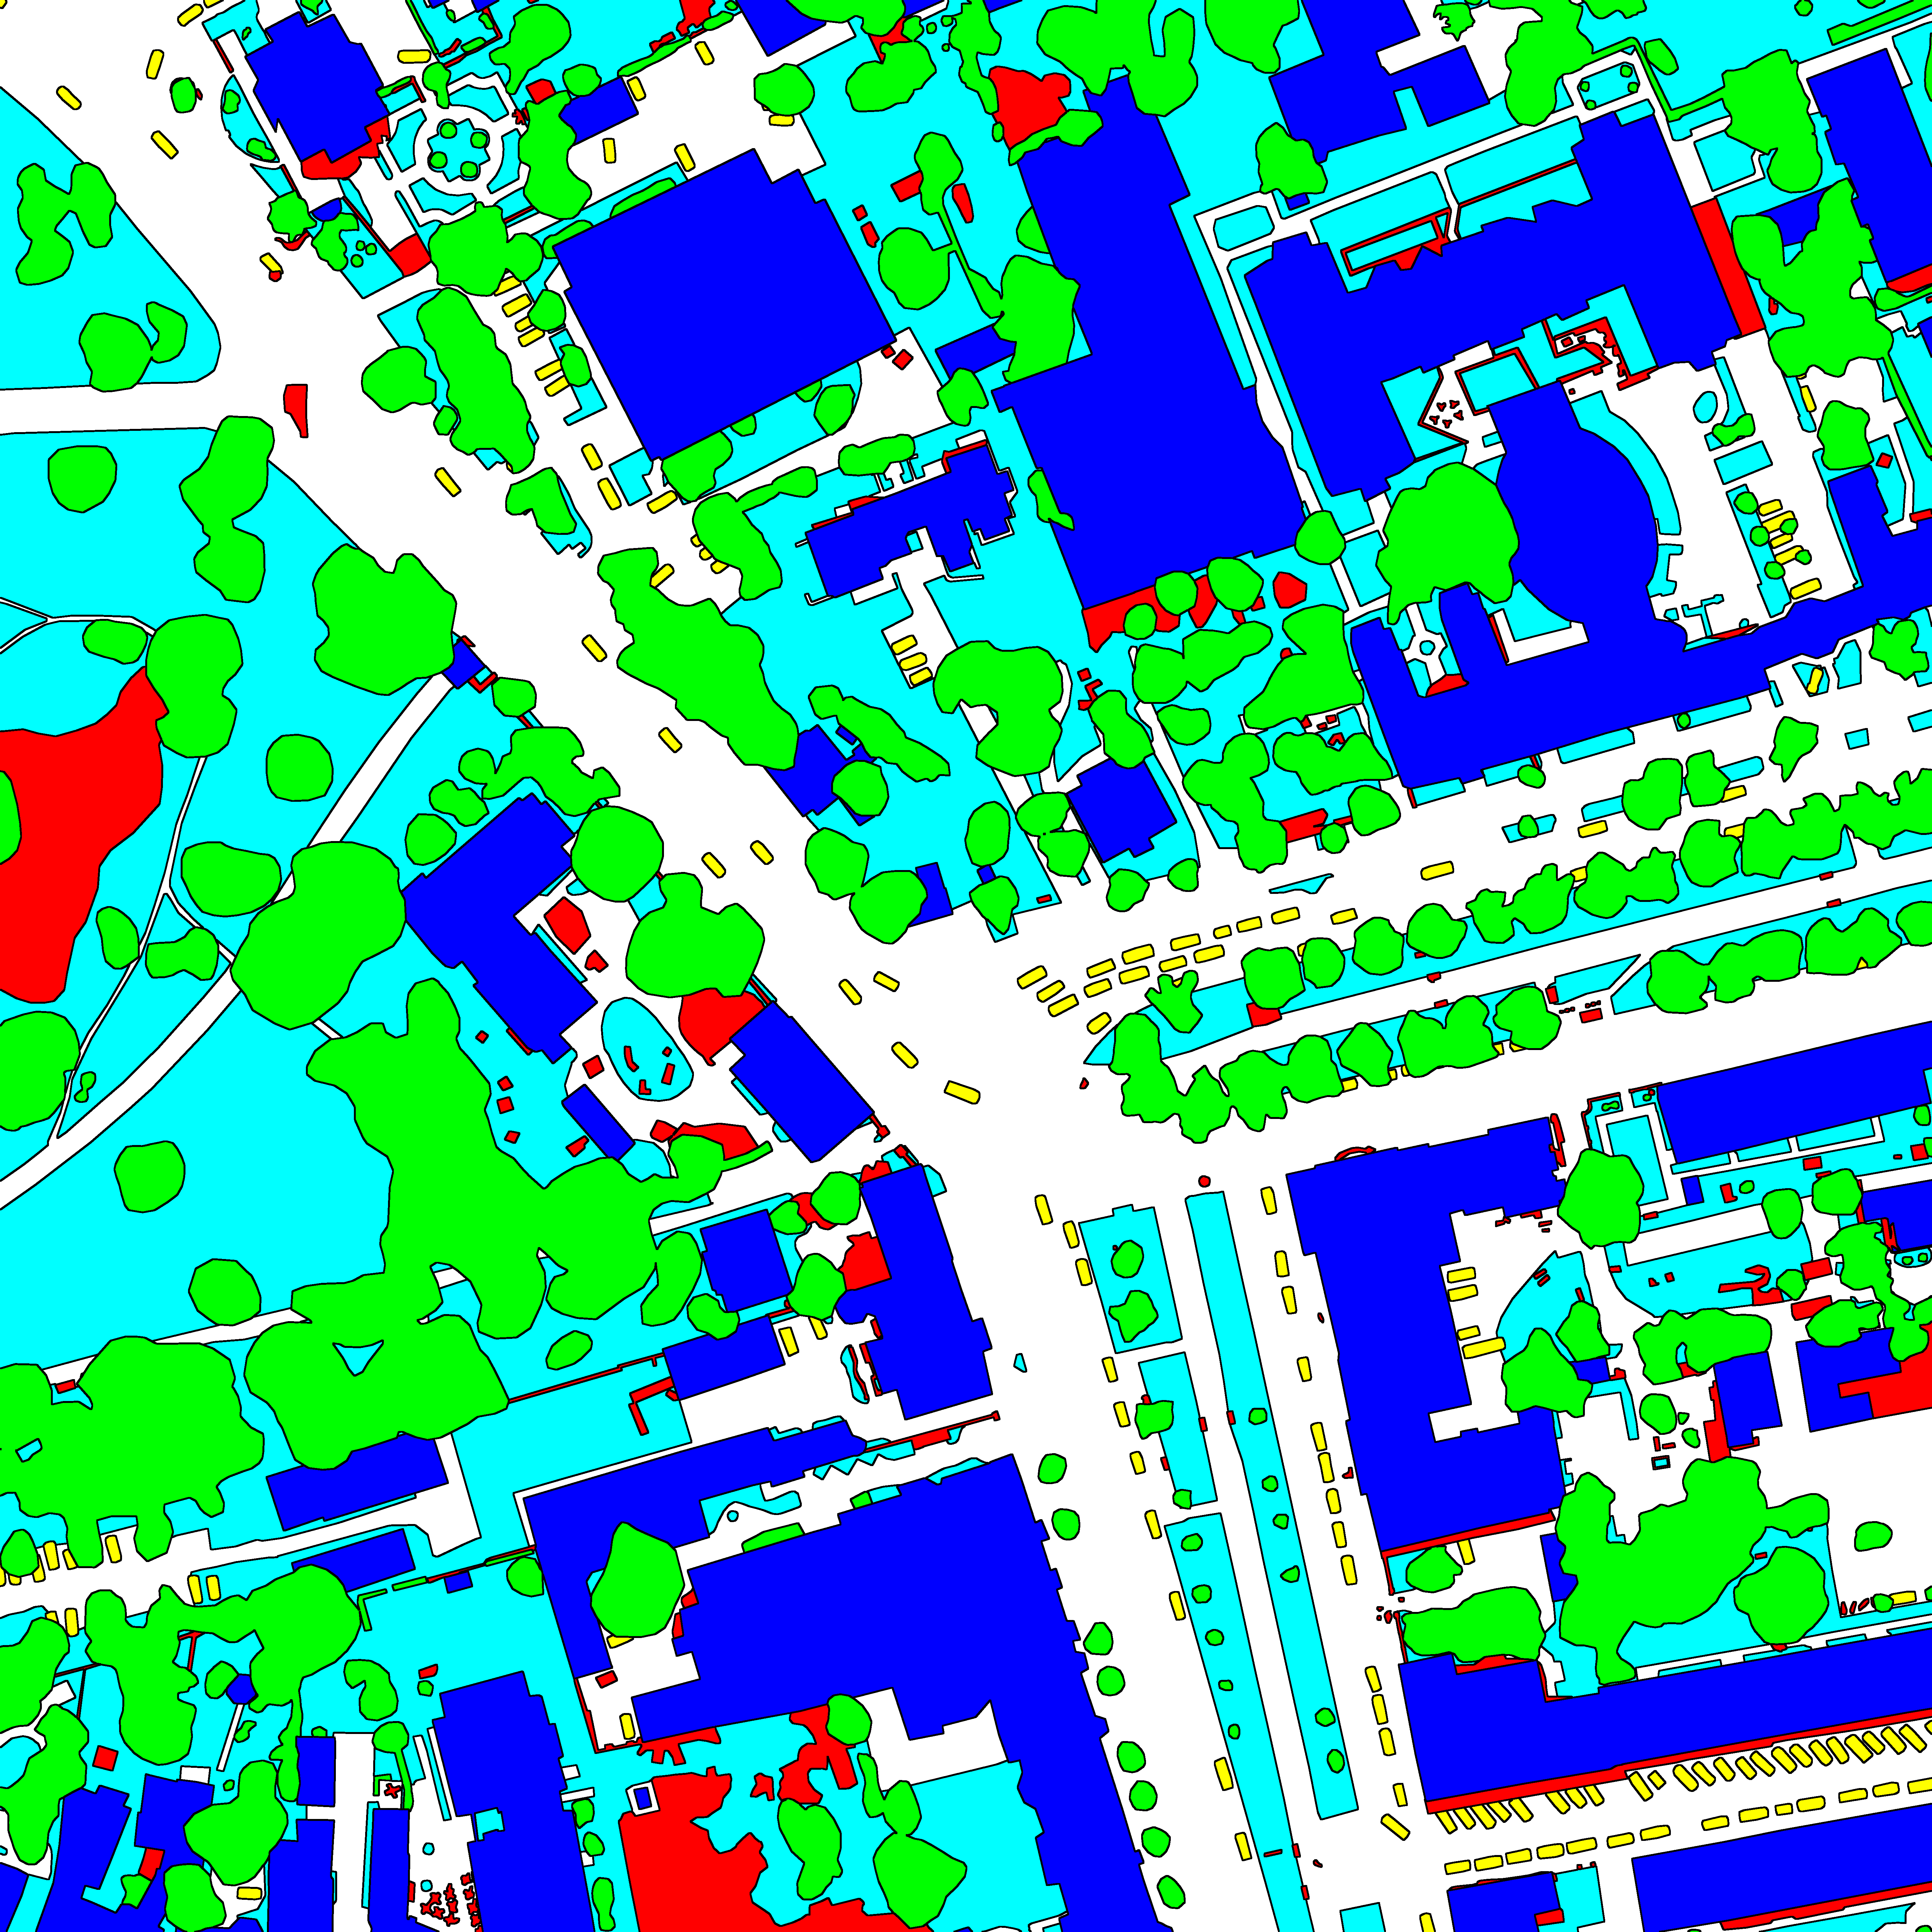
\includegraphics[width=0.95\textwidth, height=0.35\textheight]{images/potsdam-mask.png}
        \caption{A Mask From Potsdam Dataset \protect\cite{potsdam-vaihingen}}
        \label{fig:potsdam-mask}
    \end{minipage}
\end{figure}

\begin{figure}[!htb]
    \centering
    \begin{minipage}{0.5\textwidth}
        \centering
        \includegraphics[width=0.95\textwidth, height=0.35\textheight]{images/vaihingen-image.png}
        \caption{An Image From Vaihingen Dataset \protect\cite{potsdam-vaihingen}}
        \label{fig:vaihingen-image}
    \end{minipage}\hfill
    \begin{minipage}{0.5\textwidth}
        \centering
        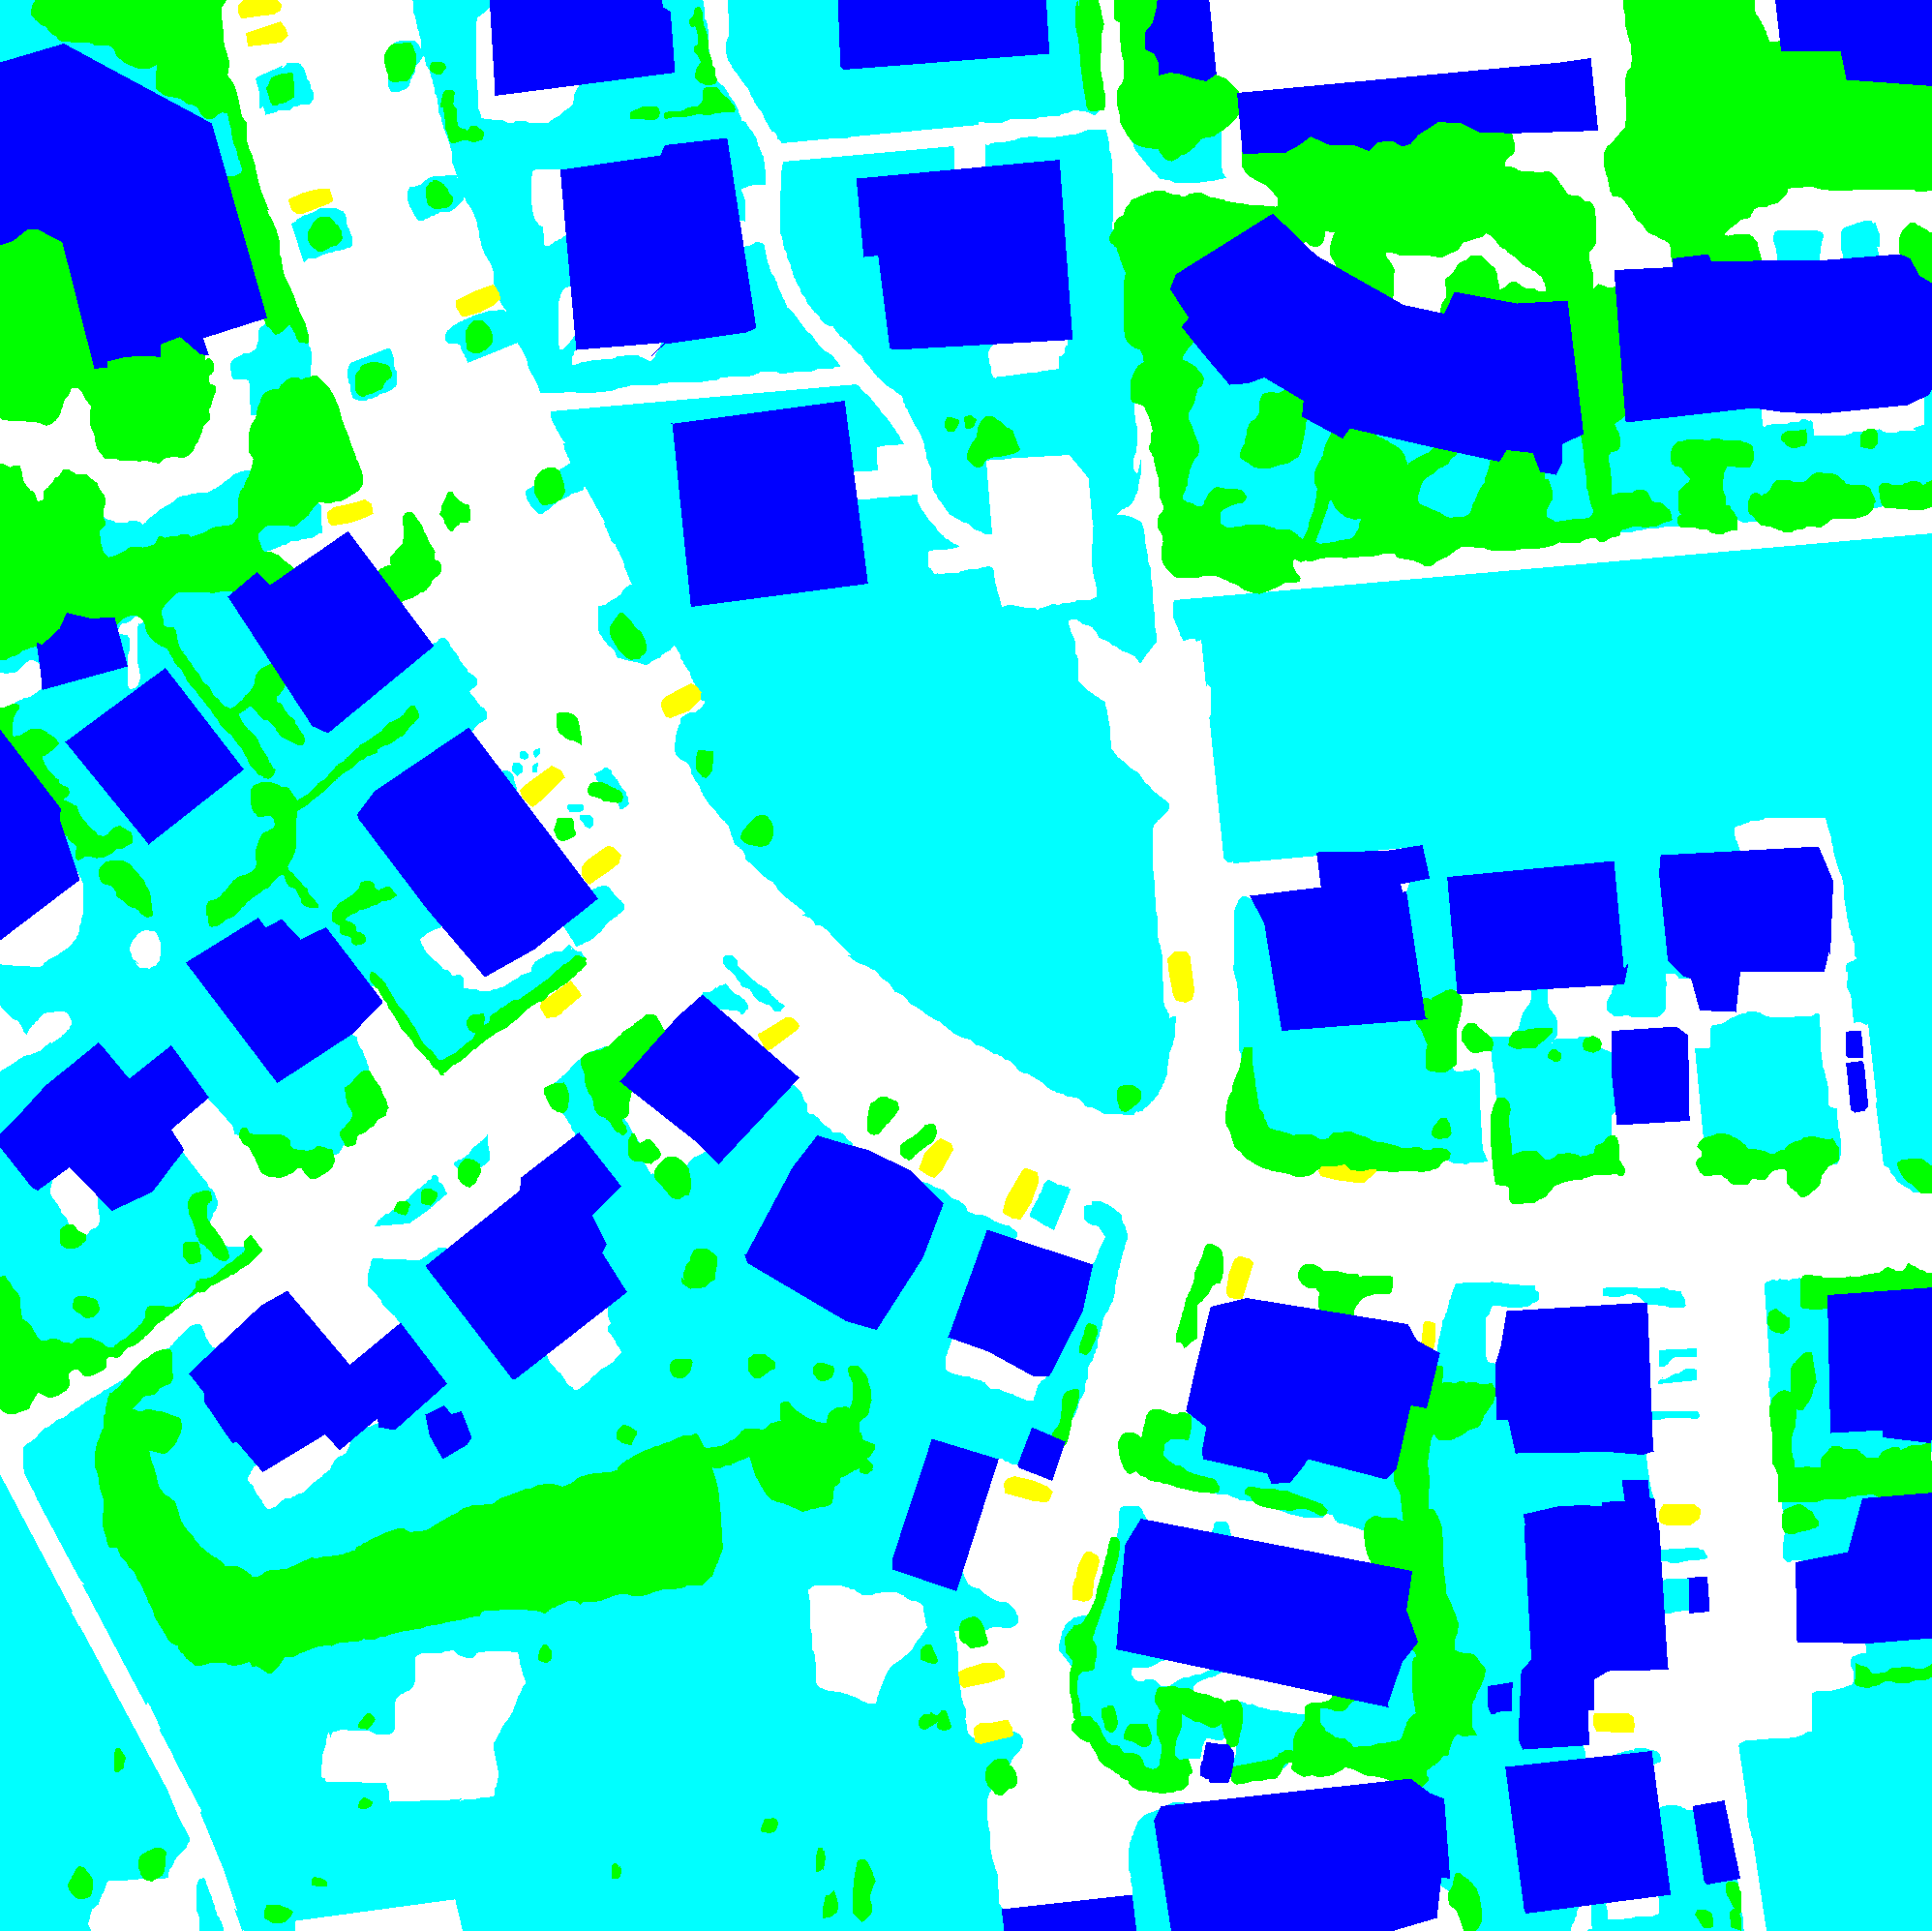
\includegraphics[width=0.95\textwidth, height=0.35\textheight]{images/vaihingen-mask.png}
\centering
\caption{A Mask From Vaihingen Dataset \protect\cite{potsdam-vaihingen}}
\label{fig:vaihingen-mask}
    \end{minipage}
\end{figure}


\FloatBarrier

%%%%%%%%%%%%%        LoveDA             %%%%%%%%

The LoveDA dataset \cite{loveda} contains 5987 High Spatial Resolution (HSR) images with 166768 annotated pixels from three different cities in China. The images are obtained from Google Earth. The images are divided into two sub-categories: urban and rural. There are nine urban areas selected from different economically developed districts, which are all densely populated. The other nine rural areas were selected from undeveloped districts. The spatial resolution is 0.3 m, with
red, green, and blue bands. After geometric registration and pre-processing, each area is covered by 1024 × 1024 images, without overlap. LoveDA dataset contains a total of 7 classes: building, road, water, agriculture, barren, forest and background. Figure \ref{fig:loveda-image} and \ref{fig:loveda-mask} shows a pair of an image and its corresponding mask from LoveDA dataset.

\FloatBarrier
\begin{figure}[!htb]
    \centering
    \begin{minipage}{0.5\textwidth}
        \centering
        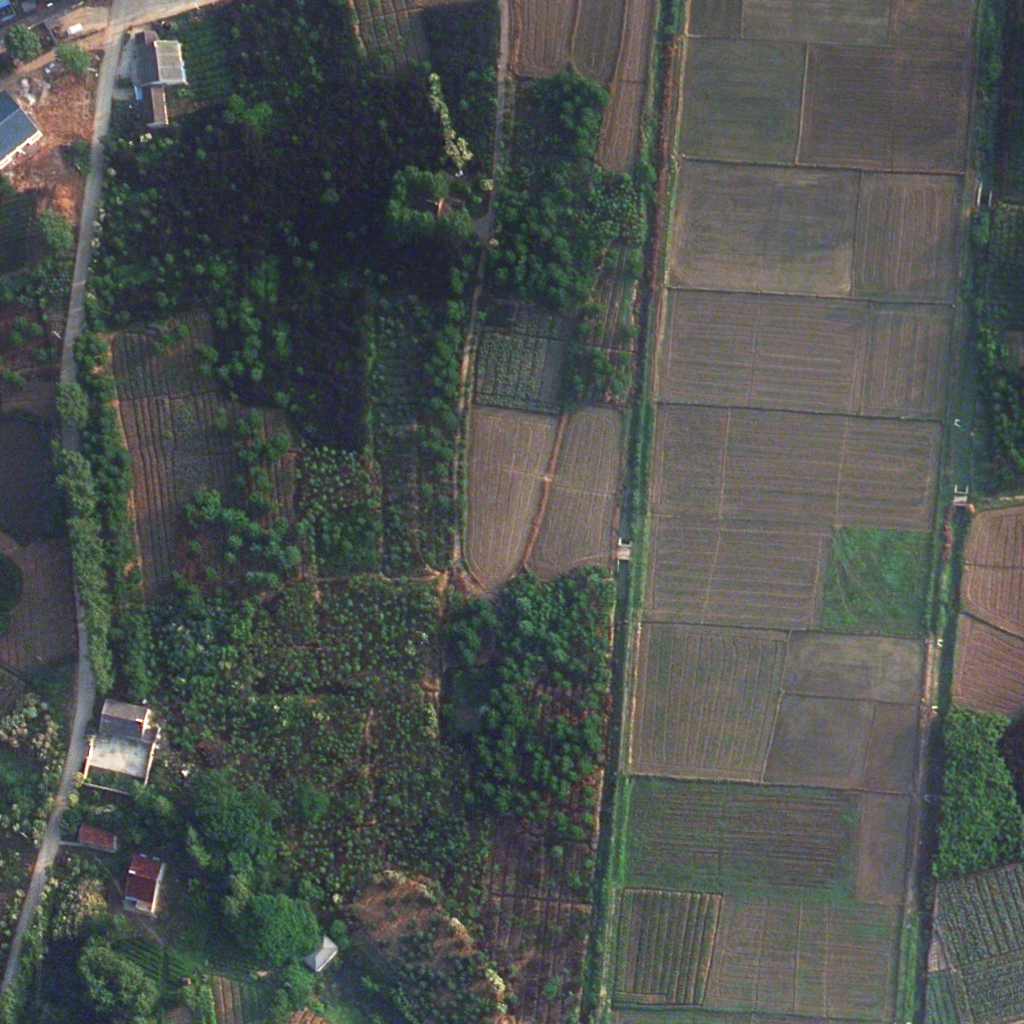
\includegraphics[width=0.95\textwidth, height=0.35\textheight]{images/loveda-image.png}
        \caption{An Image From LoveDa Dataset \protect\cite{loveda}}
        \label{fig:loveda-image}
    \end{minipage}\hfill
    \begin{minipage}{0.5\textwidth}
        \centering
        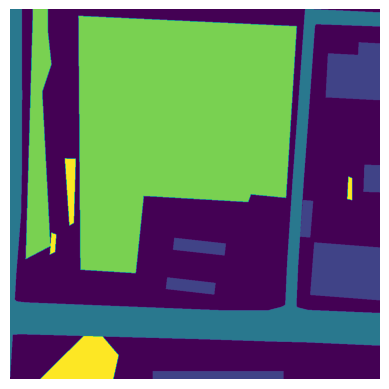
\includegraphics[width=0.95\textwidth, height=0.35\textheight]{images/loveda-mask.png}
\centering
\caption{A Mask From LoveDa Dataset \protect\cite{loveda}}
\label{fig:loveda-mask}
    \end{minipage}
\end{figure}
\FloatBarrier


%%%%%%%GID%%%%%%%%%%%%
The GID-5 dataset \cite{GID2020} contains 120 6800 x 7200 HSR images with 5 classes. The classes are built-up, farmland, meadow, farmland and water which are pixel-level labeled with five different colors: red, green, cyan, yellow,
and blue, respectively. The images are obtained from Gaofen-2 satellite. GID-5 dataset is widely distributed over the geographic areas covering more than 50,000 $km^2$. Due to the extensive geographical distribution, GID-5 represents the distribution information of ground objects in different areas. Figure \ref{fig:gid-image} and \ref{fig:gid-mask} shows an example of an image and its corresponding mask from Deep Globe dataset.

\FloatBarrier
\begin{figure}[!htb]
    \centering
    \begin{minipage}{0.5\textwidth}
        \centering
        \includegraphics[width=0.95\textwidth, height=0.35\textheight]{images/gid image.png}
        \caption{An Image From GID-5 Dataset \protect\cite{GID2020}}
        \label{fig:gid-image}
    \end{minipage}\hfill
    \begin{minipage}{0.5\textwidth}
        \centering
        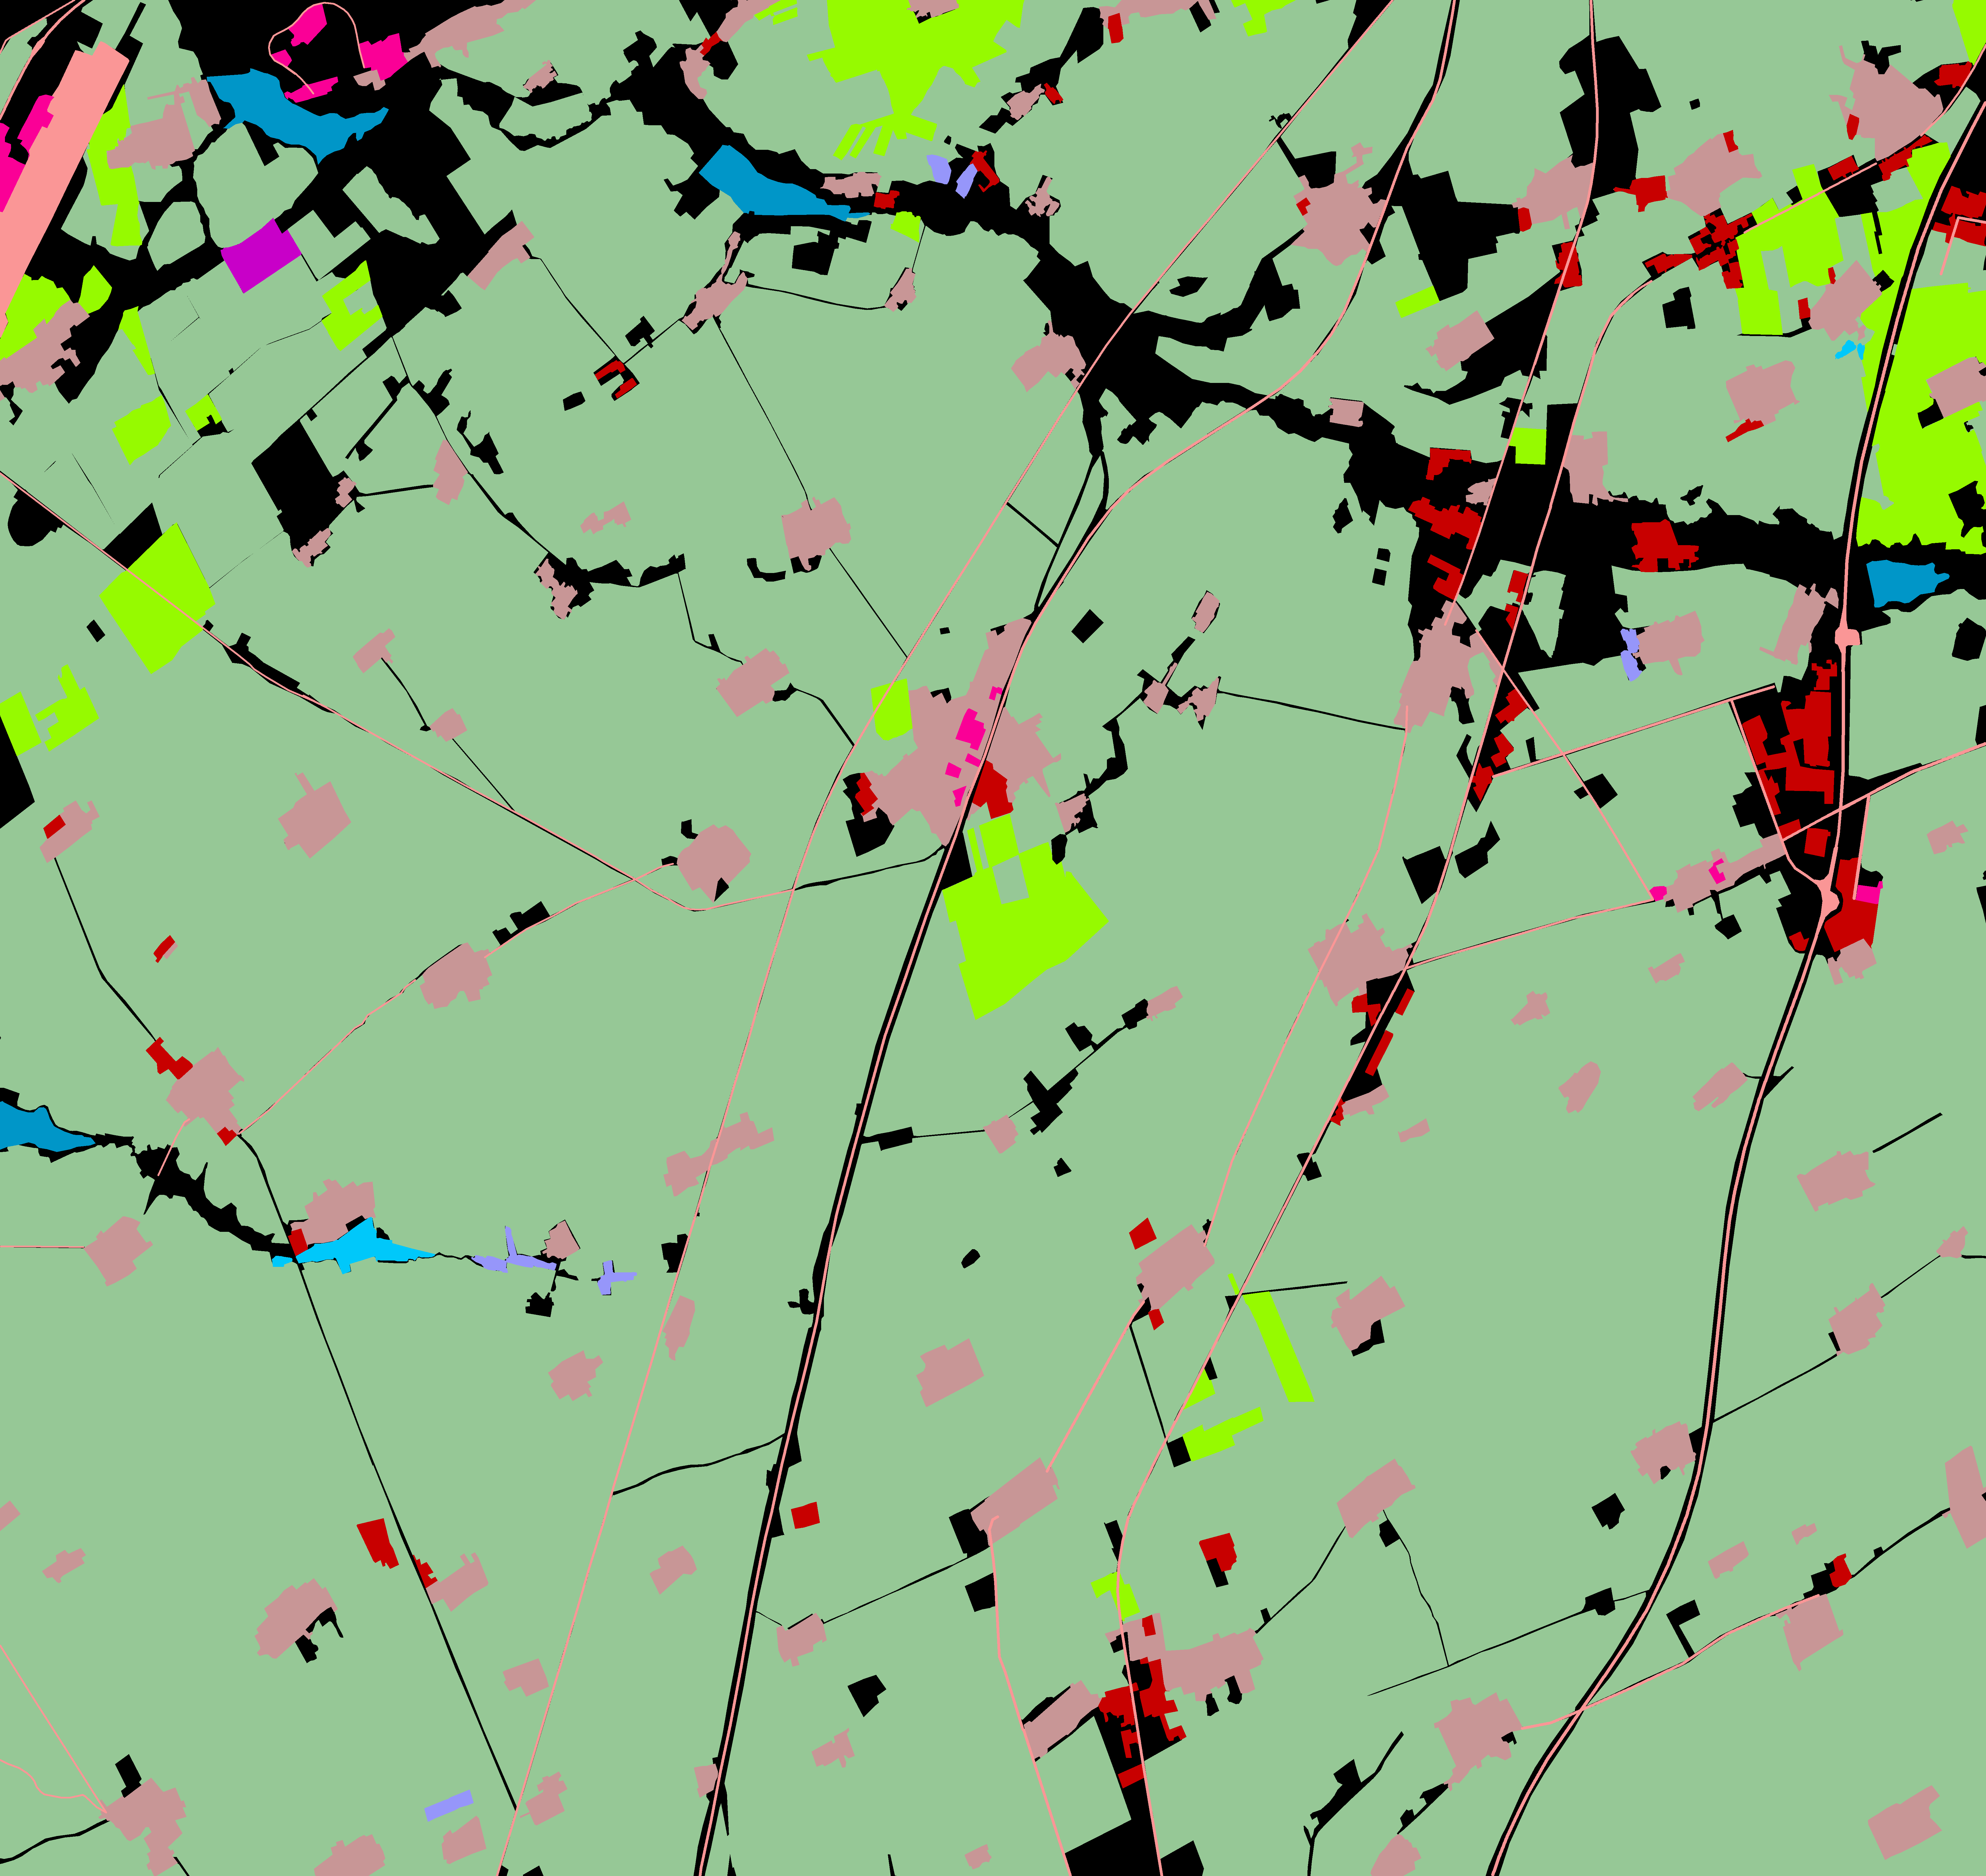
\includegraphics[width=0.95\textwidth, height=0.35\textheight]{images/gid mask.png}
\centering
\caption{A Mask From GID-5 Dataset \protect\cite{GID2020}}
\label{fig:gid-mask}
    \end{minipage}
\end{figure}
\FloatBarrier


%%deep-globe%%%
The Deep Globe Land Cover dataset \cite{deep-globe} contains 1146 satellite images of size 2448×
2448 pixels. The dataset is split into training, validation and test sets, each with 803/171/172 images. All images contain RGB channel, with a pixel resolution of 50 cm. The dataset is  collected from the DigitalGlobe Vivid+ dataset which is an earlier dataset containing satellite images. The annotations are pixel-wise segmentation masks created by professional annotators. There are 7 total classes:

\begin{enumerate}
    \item Urban land: Man-made, built up areas with human artifacts.
    \item Agriculture land: Farms, plantation, cropland, orchards, vineyards, nurseries, and ornamental horticultural areas; confined feeding infrastructure.
    \item Rangeland: Any non-forest, non-farm, green land, grass.
    \item Forest land: Any land with at least 20\% tree crown density plus clear cuts.
    \item Water: Rivers, oceans, lakes, wetland, ponds.
    \item Barren land: Mountain, rock, dessert, beach, land with no vegetation.
    \item Unknown: Clouds and others.
\end{enumerate}


Figure \ref{fig:deep-globe-image} and \ref{fig:deep-globe-mask} shows an example of an image and its corresponding mask from Deep Globe dataset.


\FloatBarrier
\begin{figure}[!htb]
    \centering
    \begin{minipage}{0.5\textwidth}
        \centering
        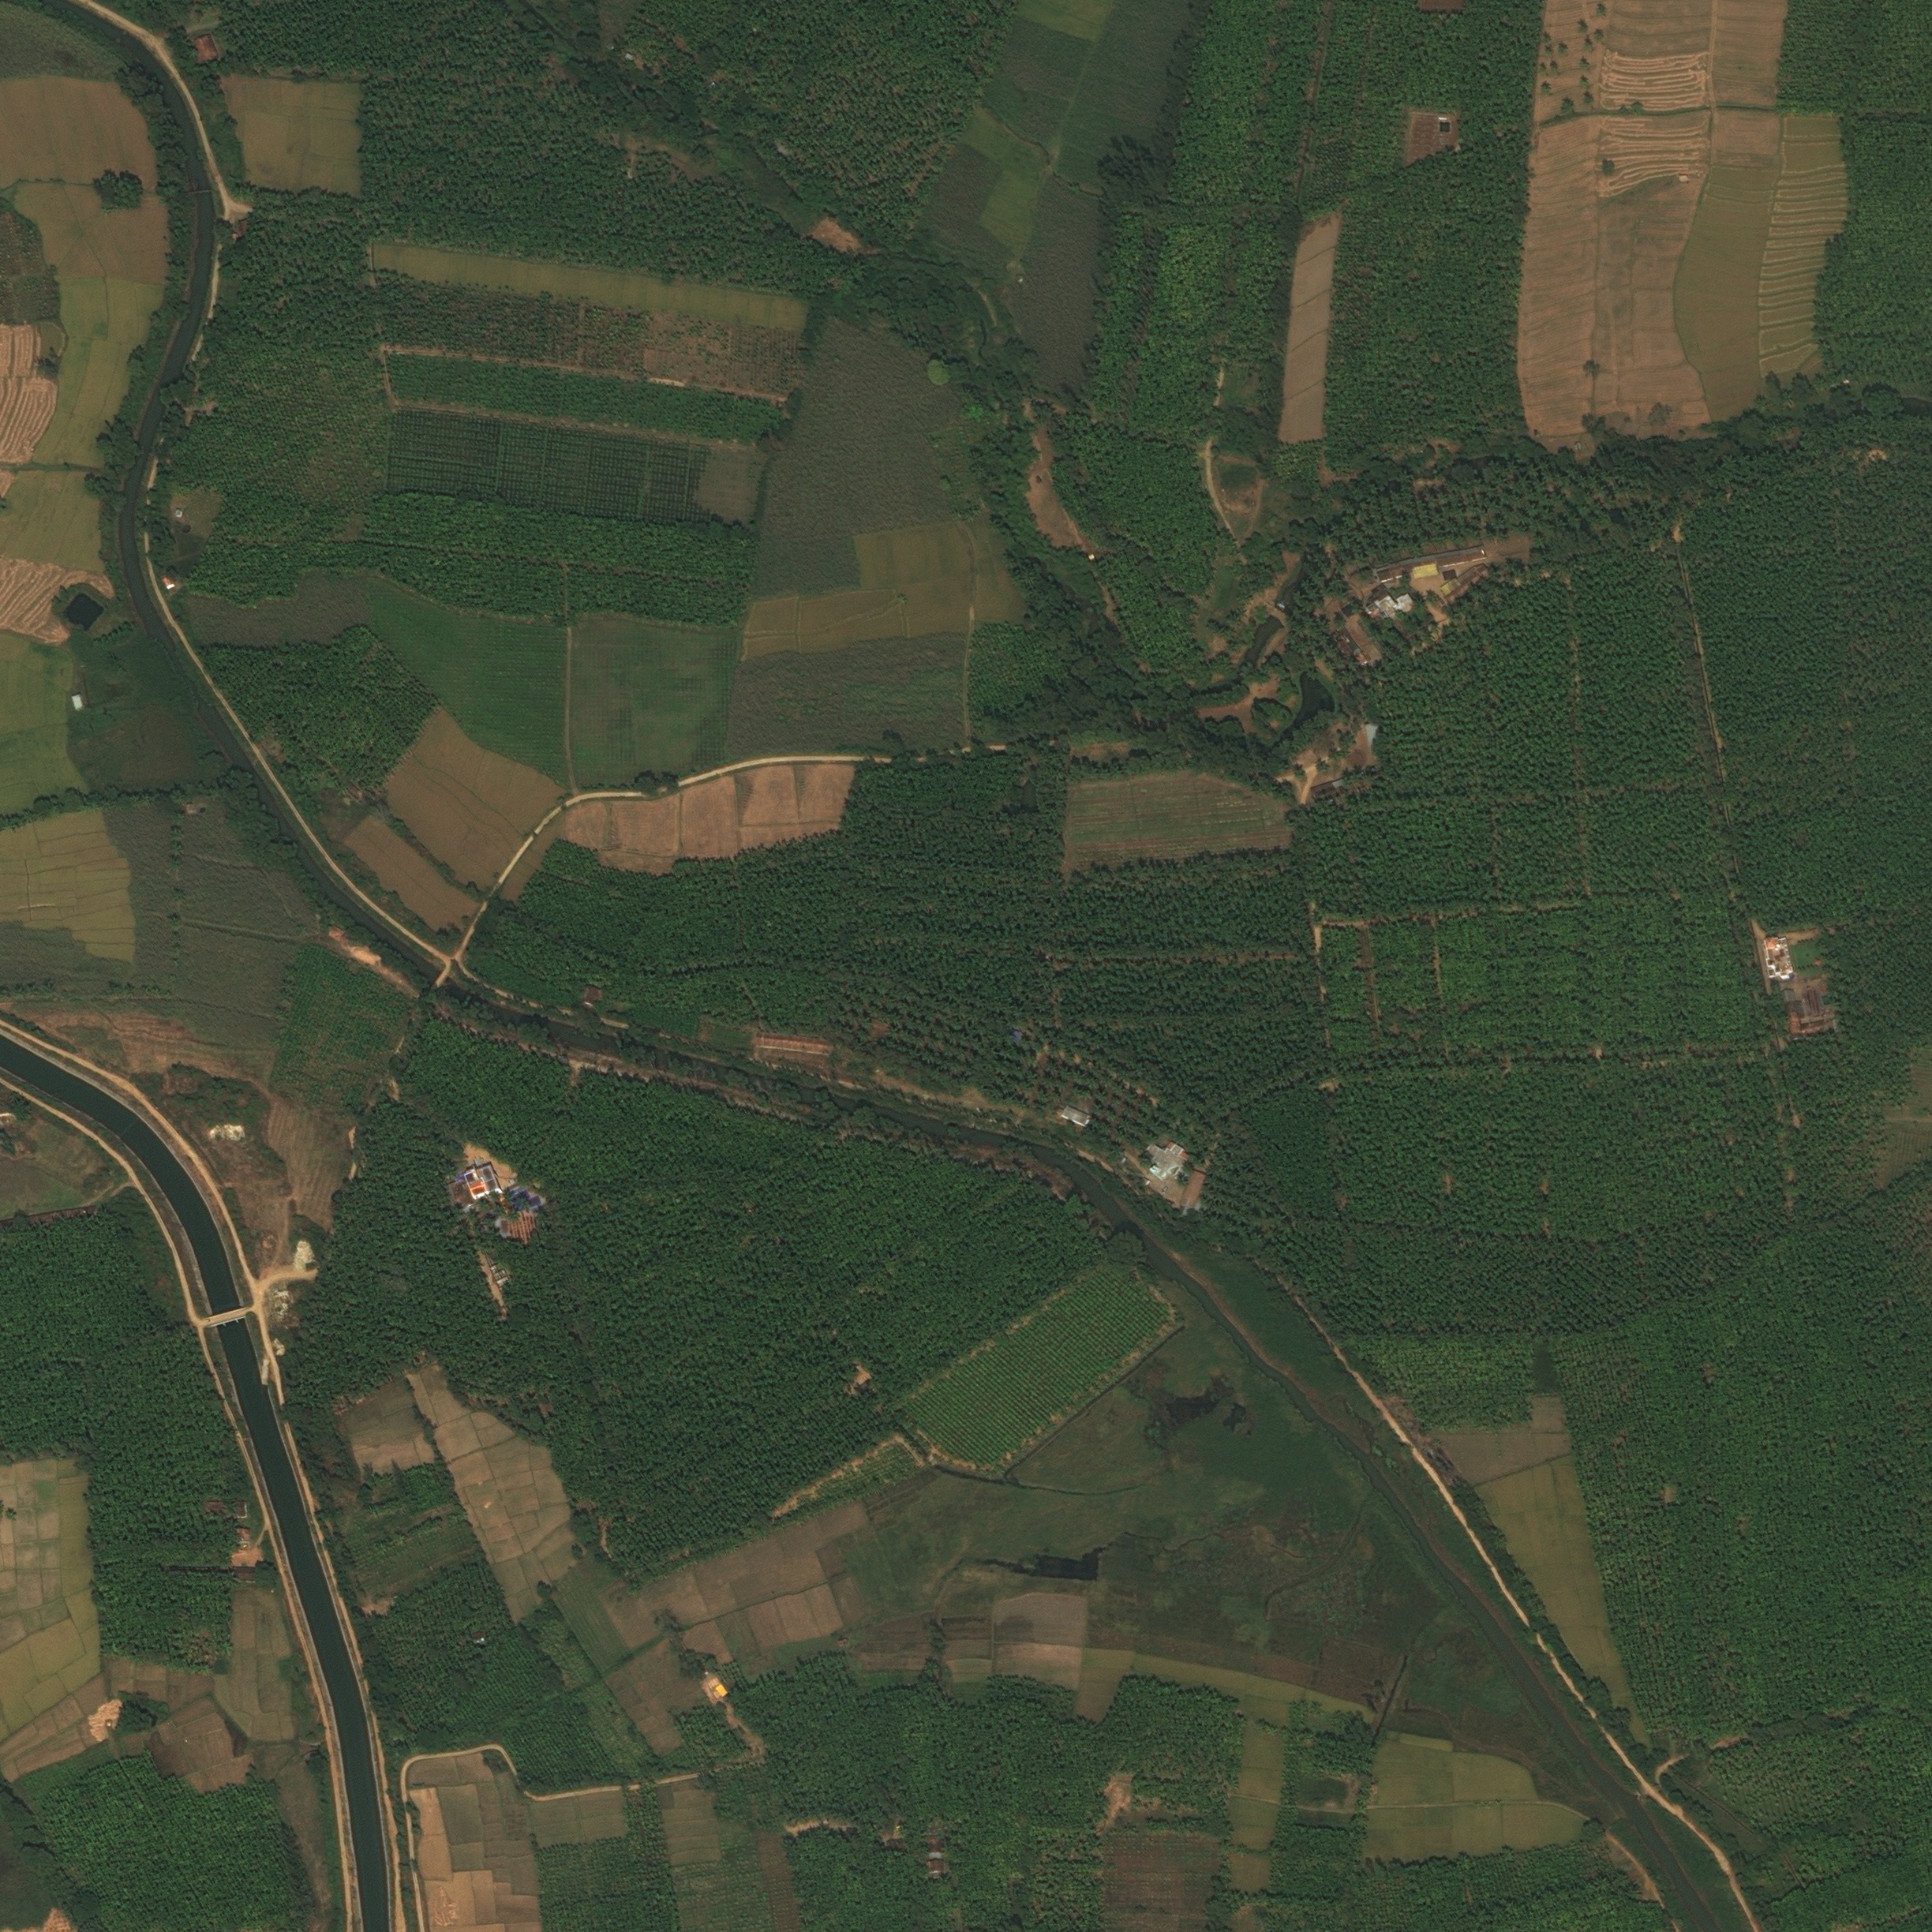
\includegraphics[width=0.95\textwidth, height=0.35\textheight]{images/deepglobe_img.jpg}
        \caption{An Image From Deep Globe Dataset \protect\cite{deep-globe}}
        \label{fig:deep-globe-image}
    \end{minipage}\hfill
    \begin{minipage}{0.5\textwidth}
        \centering
        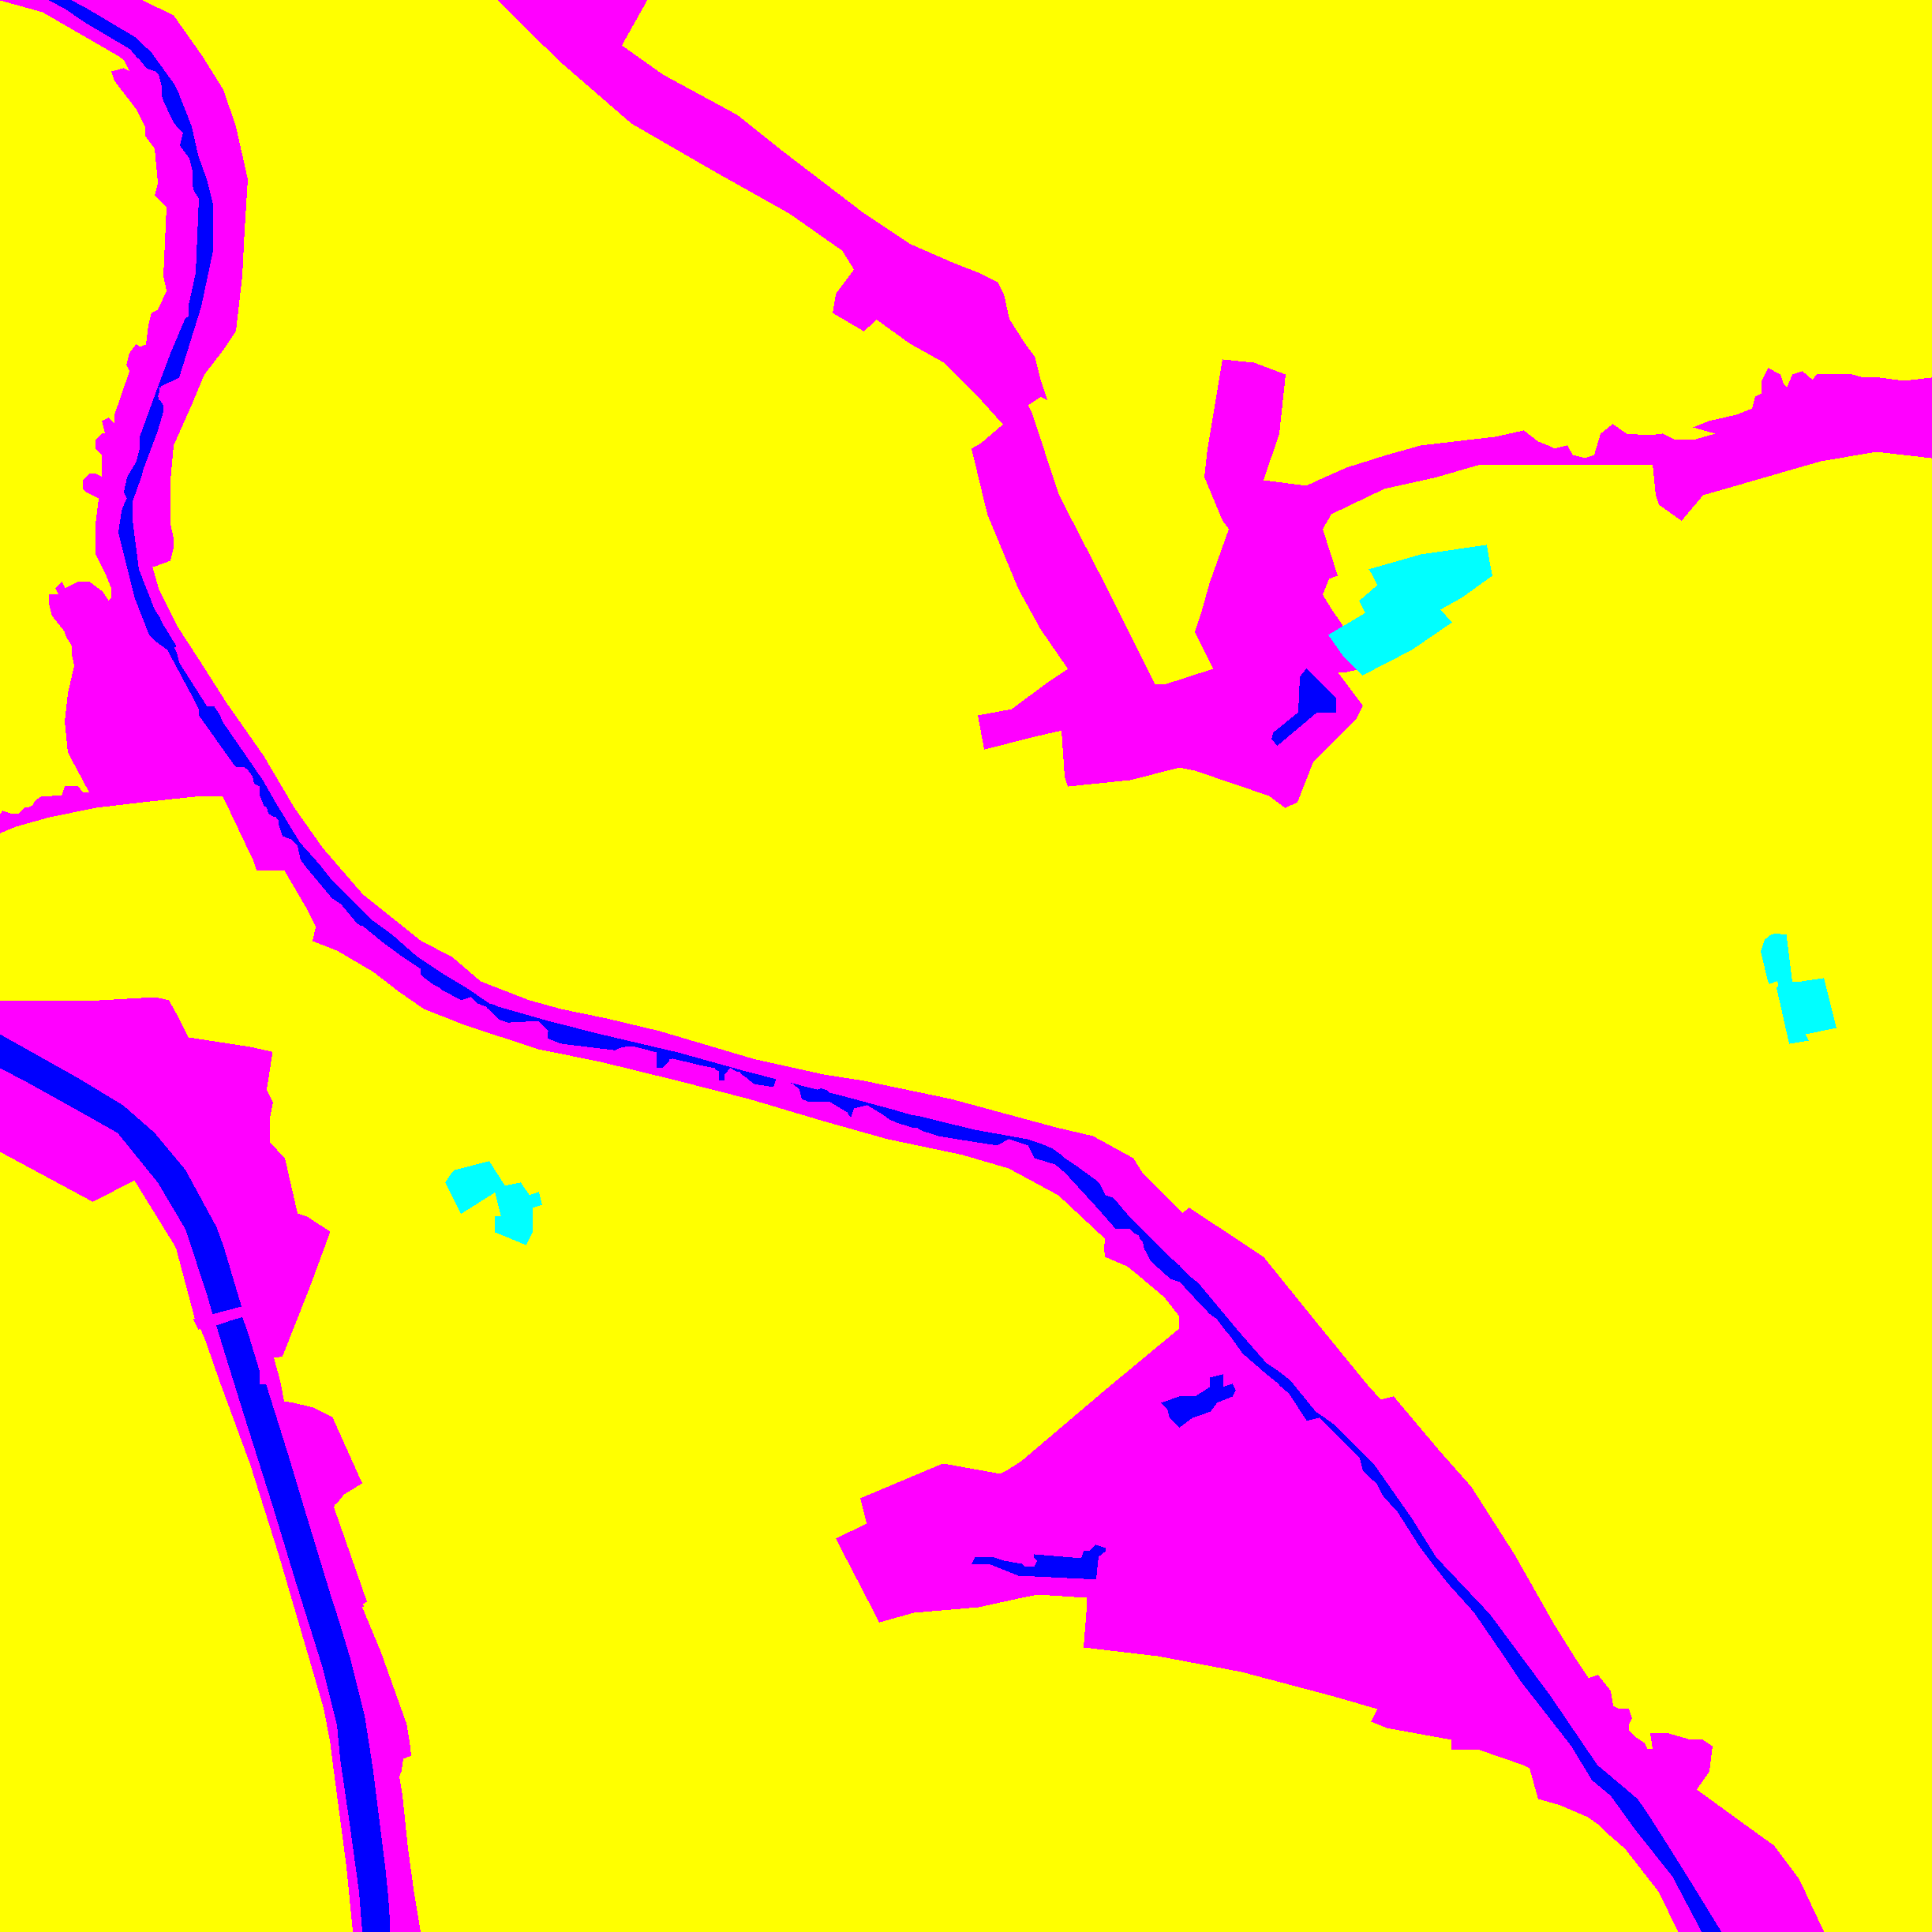
\includegraphics[width=0.95\textwidth, height=0.35\textheight]{images/deepglobe_mask.png}
\centering
\caption{A Mask From Deep Globe Dataset \protect\cite{deep-globe}}
\label{fig:deep-globe-mask}
    \end{minipage}
\end{figure}
\FloatBarrier



The LandCover.ai dataset \cite{landcoverai} is a simple RGB-only dataset with spatial resolution of 25 or 50 cm per pixel. There are 33 images with resolution 25 cm(9000 × 9500 px) and 8 images with resolution 50 cm (4200 × 4700 px). Pixel-wise annotations are made manually with VGG Image Annotator (VIA) by a group of people using polygon shape and polylines. LandCover.ai dataset has 5 classes: buildings, woodlands, water, roads and background. Figure \ref{fig:landcover-image} and \ref{fig:landcover-mask} show a pair of its image and mask.

\FloatBarrier
\begin{figure}[!htb]
    \centering
    \begin{minipage}{0.5\textwidth}
        \centering
        \includegraphics[width=0.95\textwidth, height=0.35\textheight]{images/landcoverai-image.jpg}
        \caption{An Image From Deep Landcover.ai Dataset \protect\cite{landcoverai}}
        \label{fig:landcover-image}
    \end{minipage}\hfill
    \begin{minipage}{0.5\textwidth}
        \centering
        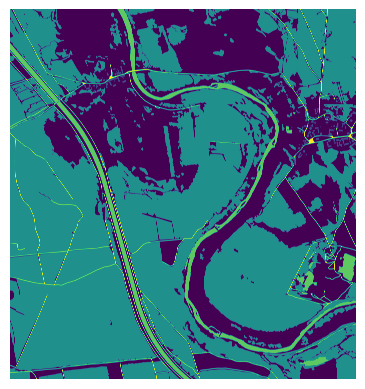
\includegraphics[width=0.95\textwidth, height=0.35\textheight]{images/landcoverai-mask.png}
\centering
\caption{A Mask From Landcover.ai Dataset \protect\cite{landcoverai}}
\label{fig:landcover-mask}
    \end{minipage}
\end{figure}
\FloatBarrier




\section{Semantic Segmentation Before Deep Learning}

This section would elaborate on traditional methods of semantic segmentation, methods that do not apply any neural networks for semantic segmentation. Before deep learning, semantic segmentation relied heavily on feature extraction and traditional machine learning (ML) algorithm as shown in Figure \ref{fig:trad}. These two methods are rendered obsolete by deep learning.

\FloatBarrier
\begin{figure}[ht]
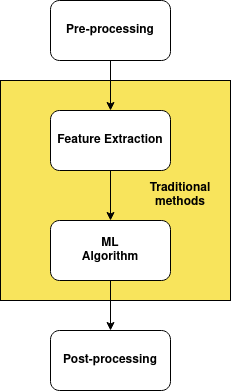
\includegraphics[width=5.5cm, height=7.5cm]{images/traditional.png}
\centering
\caption{Semantic Segmentation Before Deep Learning.}
\label{fig:trad}
\end{figure}
\FloatBarrier


\subsection{Feature Extraction}
Before we apply any of the traditional ML algorithm that will be discussed in the proceeding sections  we must extract the features from an image. The accuracy of traditional semantic segmentation methods heavily depends on the selected features. The features may be the numerical value of each pixel or the feature map containing the gradient of each pixel. There are three feature extraction methods discussed in this section, namely they are Histogram of Oriented Gradients, Scale-Invariant Feature Transform and Bag of Visual Words .

\begin{enumerate}
    \item \textbf{\textit{Histogram of Oriented Gradients (HOG).}} HOG features interpret any given image as a discrete function $I : \mathbb{N}^2 \rightarrow \{0...255\}$ that maps a pair value $(x,y)$ which is the coordinate of the pixel to an RGB value. Then, the partial derivative in of \(x\) and \(y\) are calculated for every pixel. The input image is now transformed into a feature map with the gradient of each pixel. Lastly, the constructed feature map is divided into smaller patches and the direction and magnitude of the histogram is calculated for each patch. \cite{DBLP:journals/corr/Thoma16a}.

    \begin{figure}[ht]
    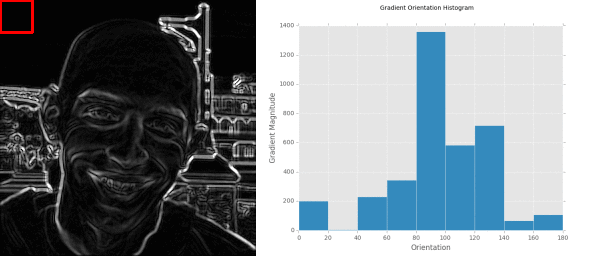
\includegraphics[width=12cm, height=6cm]{images/hog.png}
    \centering
    \caption{Computing a histogram of oriented gradients for the first patch of an input image.}
    \label{fig:hog}
    \end{figure}
    
    \item \textbf{\textit{Scale-Invariant Feature Transform (SIFT).}} SIFT is a feature extraction algorithm that was introduced in 2004. Unlike HOG, SIFT is not affected by the orientation or scale of the input image. \cite{DBLP:journals/corr/Thoma16a}. An image will be divided into smaller patches and the difference-of-Gaussian (DoG)is calculated. DoG is obtained as the difference of Gaussian blurring of an image with two different $\sigma$. Next, local extrema is searched to be be assigned as potential key points. Lastly, after the key points are discovered, an 8-bin orientation histogram is created for each patch to math the key points. The final output will be a feature map containing accepted key points. A more thorough explanation is available in the original paper \cite{SIFT}.

    \begin{figure}[ht]
    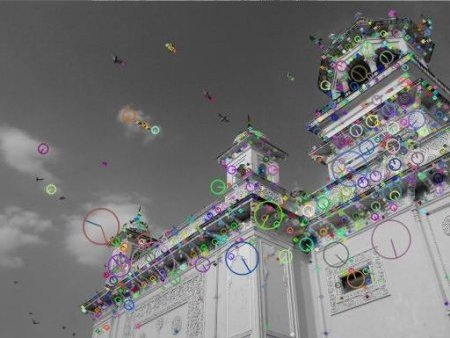
\includegraphics[width=12cm, height=7.5cm]{images/sift_keypoints.jpg}
    \centering
    \caption{Each circle represents the location and orientation of SIFT keypoints}
    \label{fig:sift_keypoints}
    \end{figure}

    
    \item \textbf{\textit{Bag of Visual Words (BOV).}} BOV construct sparse histograms that contain the frequency of features in an image. Those features are usually extracted using SIFT \cite{DBLP:journals/corr/Thoma16a}. BOV is often used alongside other feature extractors such as SIFT by assigning each SIFT descriptor to the closest entry in a visual dictionary.
\end{enumerate}

\subsection{Traditional Machine Learning Algorithm}
\subsubsection{Random Decision Forest for Semantic Segmentation}
 A decision tree is a tree where each leaf represents a class and each non-leaf nodes uses the feature inputs to decide which branch to descend to \cite{DBLP:journals/corr/Thoma16a}. A random decision tree is as decision tree that is injected with some randomness during the training phase  to reduce over-fitting and increase accuracy. Random Decision Forest is an unsupervised ensemble learning method that are made up of multiple independently constructed random decision trees. An in-depth explanation to semantic segmentation using Random Decision Forest is given by \cite{Schroff2008ObjectCS}. 
 
\subsubsection{Support Vector Machines (SVM) for Semantic Segmentation}

In SVM the training data is represented as $(x_i,y_i)$ where $x_i$ is the feature vector, $y_i \in \{-1,1\}$ is the class label and $i \in \{1...m\}$ where m is the number of inputs.

Assuming that the data is linearly separable, SVM is a task of solving the optimal margin classifier:

\begin{equation}
    min_{w,b} \quad \frac{1}{2}||w||^2 \\
\end{equation}

\begin{equation}
    s.t. \quad y^{i}(w^T x^i +b)\geqslant 1, i \in {1...m}
\end{equation}

\vspace{0.1cm}

Where $w$ is the weight, $x$ the input vector, $y$ is the output vector and $b$ is the bias. $w$can be defined as:

\begin{equation}
    w = \sum_{i=1}^m \alpha_i y_i x_i
\end{equation}

Where $\alpha$ is the Lagrange multiplier.

Not every dataset is linearly separable thus this problem can be solved by transforming the feature vectors $x$ into a higher dimension using a non-linear mapping $/psi$. Thus instead of learning using $x$, we may learn using a higher-dimensional features generated by $\psi(x)$, this method is called the \textit{kernel trick}. Specifically, given a feature mapping $\psi$, we define the corresponding kernel to be:    

\begin{equation}
    K(x,z)=\psi(x)^T\psi(z)
\end{equation}

The SVM described above can only distinguish between binary classes.The one-vs-all strategy and the one-vs-one strategy are methods used to expand it to be a multi-class classifier.. In the one-vs-all strategy n classifiers have to be trained which can distinguish one of the n classes against all other classes. In the one-vs-one strategy $\frac{n^2-n}{2}$ classifiers are trained; one classifier for each pair of classes.

\subsubsection{Markov Random Field (MRF)} MRF maps an image onto an undirected graph where each node is a pair of random variable $(x,y)$ assigned to each pixel and the edges connect adjacent pixels \cite{YU201882}. $x$ represents the class label of a pixel and $y$ represents the RGB value of a pixel. Which means $x$ has a range of ${0...n}$ and y has a range of ${0...255}$ with $n$ being the number of classes.  Every edge is assigned conditional dependencies of its connecting nodes as weight. The probability of $x,y$ can be expressed as:

\begin{equation}
    P(x,y) = \frac{1}{Z} e^{-E(x,y)
\end{equation}

Where $Z = \sum_{x,y}e^{-E(x,y)}$ and it is called the partition function and $E$ is the energy function. A commonly used energy function is $E(x,y) = \sum_{c\in C}\psi_{c}(x,y)$, where $\psi$ is called the clique potential \cite{DBLP:journals/corr/Thoma16a}. A thorough presentation of MRF can be found in \cite{markovbook}. 

\subsubsection{Conditional Random Field (CRF) for Semantic Segmentation} CRF is an extension of MRF. Instead of learning the distribution $P(x,y)$, it chooses to learn $P(x|y)$ \cite{DBLP:journals/corr/Thoma16a}. There are two advantages that CRF has over MRF. The first one being it does not to estimate the distribution of x. The second advantage is the consequence of the first one, as the distribution of x is not being estimated, less computation is required hence making CRF faster than MRF \cite{YU201882}. CRF has the partition function $Z(x)$:
\begin{equation}
    Z(x) = \sum_{x} P(x,y)
\end{equation}

\noindent and the joint probability distribution is given as follows:

\begin{equation}
    P(y|x) = \frac{1}{Z(x)} \prod_{c \in C}\psi_{c}(y_{c}|x)
\end{equation}

\noindent CRF is often used in conjunction with neural networks as a post-processing method for semantic segmentation task. It is is used to smoothen the output mask \cite{crf-semantic}.

\section{Limitations of Traditional Methods}
\begin{enumerate}
    \item The traditional method is simply less accurate. As an example the best traditional method back in 2015 which utilized SIFT features extraction method and Fisher Vectors, had a performance of about 25.7\% error rate on semantic segmentation task on ILSVRC-2010 dataset. While AlexNet proposed by \cite{alexnet} had an error rate of 17.0\% \cite{DBLP:journals/corr/Thoma16a}.
    \item  Feature extraction method such as SIFT and Random Decision Forest require researchers to come up with a good hand-crafted feature to achieve high accuracy while good features are very hard to produce. Compared this with the automatically learned features provided by deep learning, traditional methods would require a lot more time and effort.

\end{enumerate}

\section{Semantic Segmentation of Satellite Images Using Convolutional Neural Networks}

Semantic segmentation task has been long dominated by Convolutional Neural network (CNN). The Fully Convolutional Network (FCN) \cite{7298965} is the first network proven to be an effective method to extract features automatically and serves as an effective end-to-end CNN structure for semantic segmentation task. The outcome of FCN, although encouraging, appears to be coarse due to the over-simplified design of the decoder.

To tackle this problem, better CNNs were proposed such as U-Net \cite{unet} which  introduced the encoder-decoder framework. Since its introduction, the encoder-decoder framework has become the standard structure of satellite images segmentation network \cite{unetformer}. U-Net introduced two symmetric paths: a contracting path, which is also known as the encoder to extract local features, and an expanding path which is also called the decoder, for extracting position. The encoder gradually apply convolutions and max pooling to reduce the resolution of the feature map, while the decoder extracts contextual information by progressively restoring the spatial resolution. At every level of the decoder skip connections are used to concatenate the output of the decoder with the feature maps from the encoder. Figure \ref{fig:unet} show the U-Net architecture. Benefiting from its translation equivariance and locality, U-Net enhances the semantic segmentation performance significantly and the encode-decoder framework has been a major influence towards semantic segmentation task. 

\begin{figure}[ht]
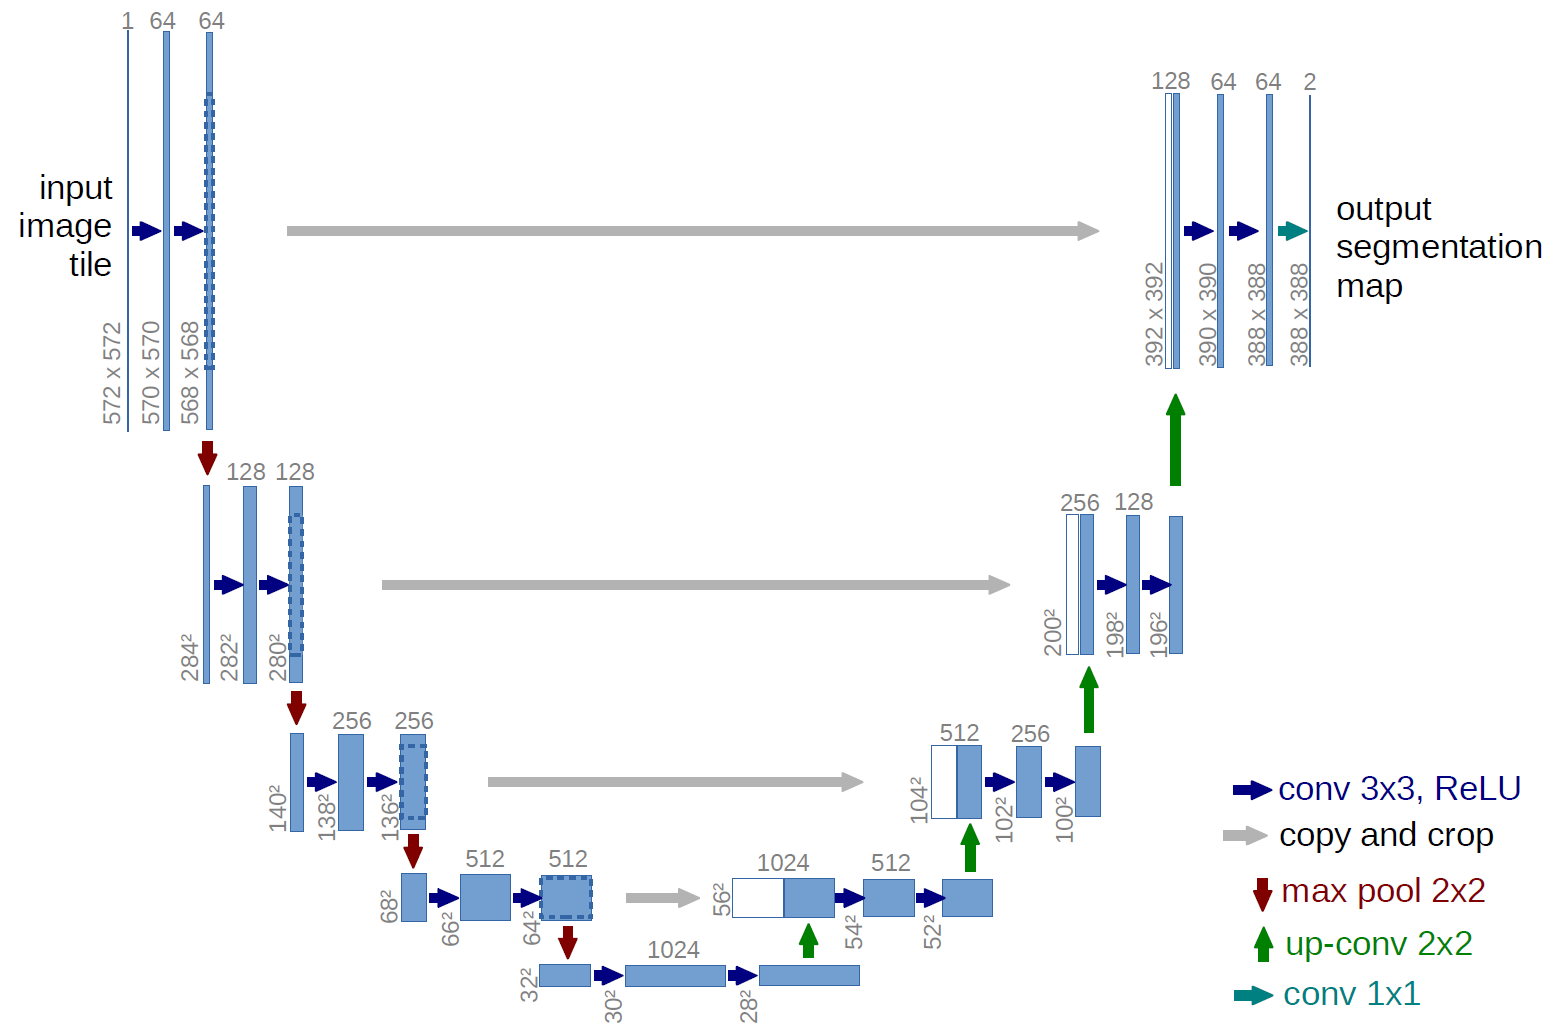
\includegraphics[width=10.5cm, height=7cm]{images/unet.png}
\centering
\caption{U-Net Architecture \protect\cite{unet}}
\label{fig:unet}
\end{figure}

Even though the results are promising, the long-range dependency of U-Net is limited by the locality property of the convolutional mechanism, which is critical for semantic segmentation. There are two types of approaches to address this issue, either modifying the convolution operation or utilizing the attention mechanism. Such examples of the first approach is to enlarge the receptive fields using large kernel sizes \cite{enlarge-receptive-field}, or utilising feature pyramids \cite{feature-pyramid}. On the other hand the second approach focuses on integrating attention mechanisms with the encoder-decoder architecture to capture long-range dependencies of the feature maps, examples can be found in Attentive Bilateral Contextual Network \cite{abcnet} and Attention U-Net \cite{attention-unet}. Although the second approach showed better performance, both approaches failed to decouple the network from the dependence of the encoder-decoder structure. In the context of semantic segmentation, per-pixel classification is often inaccurate if only local information is taken into account \cite{swin-v1}.

Attention U-Net \cite{attention-unet} is a model that aims to improve U-Net by introducing attention gates in the skip connections between the encoder and decoder as shown in \ref{fig:attention-unet}. The results showed that Attention U-Net performs better than traditional U-Net for segmentation of CT scans images.

\begin{figure}[ht]
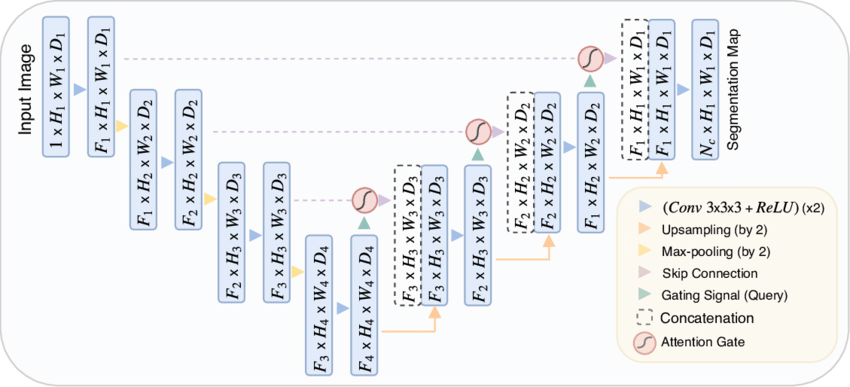
\includegraphics[width=10.5cm, height=7cm]{images/attention-unet.png}
\centering
\caption{Attention U-Net Architecture \protect\cite{attention-unet}}
\label{fig:attention-unet}
\end{figure}

U-Net with added attention mechanism is the approach favored by most literature focusing on semantic segmentation of satellite images. Multi Attention U-Net(MA-Unet) \cite{multi-attention-unet}  uses residual structure and simple attention modules. According to figure \ref{fig:maunet} the decoder in MA-Unet uses transposed convolution and attention modules at every feature fusion stage. MAUnet performed semantic segmentation task on the WHDLD datasets and DLRSD datasets. WDLD dataset have 8 classes while DLRSD dataset have 17 classes covering common classes such as farms, grasslands and lakes. MA-Unet was compareed with other U-Net based models susch as U-Net, U-Net++, Attention U-Net and MagNet on the same task. MA-Unet performs better at segmenting classes with fine details such aeroplanes. MA-Unet has the highest mIOU on both dataset with 63.94\% on WHDLD and 61.90\% on DLRSD.

Spatial Attention U-Net (SA-Unet) \cite{improved-unet} uses atrous spatial pyramid pooling as its encoder and attention modules at every skip connection like we have seen in Attention U-Net.  \cite{attention-unet-road} employs U-Net with attention to extract roads from satellite images. Instead of using simple attention modules at every skip connections, they uses attention module only once at the lowest skip connection.

\begin{figure}[ht]
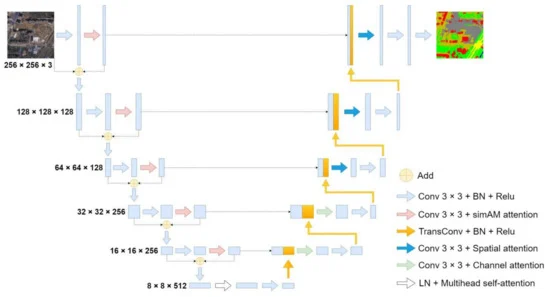
\includegraphics[width=10.5cm, height=7cm]{images/maunet.png}
\centering
\caption{Multi Attention U-Net Architecture \protect\cite{multi-attention-unet}}
\label{fig:maunet}
\end{figure}

\section{Semantic Segmentation of Satellite Images Using Vision Transformers}

Transformers were introduced by \cite{attention-is-all-you-need} and since its inception it has been the de facto model for Natural Language Processing (NLP). Transformers that are used for computer vision are called Vision Transformers to differentiate it from its NLP counterpart. Vision Transformers essentially translates 2D image-based tasks into 1D sequence-based tasks.

%%%%%benchmarking-scaling%%%%%%%
Since its inception, there are lot of researches that aim to utilize Transformers for semantic segmentation of satellite images. 
\cite{benchmarking-scaling} did a comparison of ViT, ResNet, MLPMixer and VGG trained using the BigEarthNet dataset for semantic segmentation and they concluded that ViT with a patch size of 6 delivered a slightly better performance than the rest while consuming less time to train. Interestingly, ViT with smaller patch size has lower F scores while requiring more time to train.

%%%%%%%%%%%%%%%%%%%%%%%%%%%%%  ViT
\subsection{Vision Transformer (ViT)}
Vision Transformer from \cite{16x16} is the first group of researchers that experimented with Vision Transformer by applying a standard Transformer directly to images, with the fewest possible modifications. Their model is known as Vision Transformer (ViT) as it is the first Vision Transformer. They split an image into patches, apply linear embeddings to transform the patches into vectors and provide the sequence of those linear embedding as an input to a Transformer. The image patches were treated the same way as word tokens do in an NLP application. This methods fails to capture the local context provided  CNNs hence it is unsuitable for semantic segmentation task.

Another issue with Vision Transformer is the attention mechanism itself is $O(n^2)$ because it is a dot product thus requiring it to consume significant computational time and memory to capture the global context, which in turn, reducing its efficiency, scaling potential and its potential for real-world applications. Figure \ref{fig:vit} shows the ViT architecture.

\begin{figure}[ht]
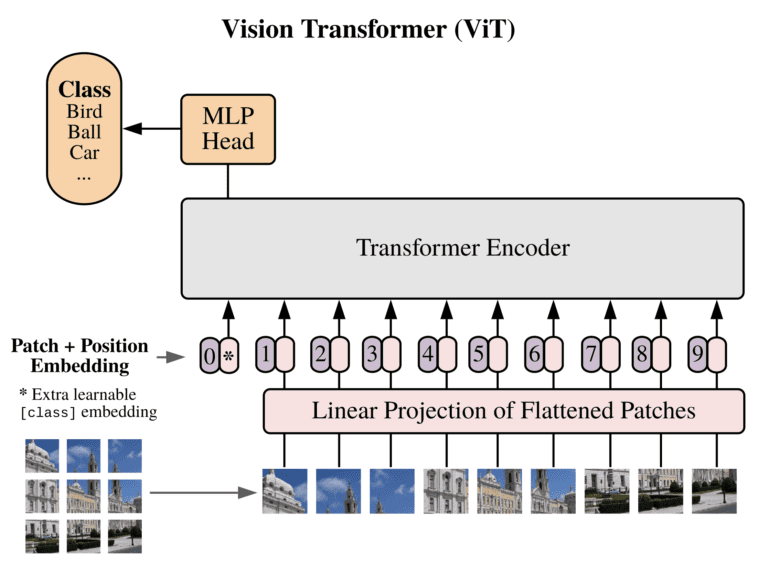
\includegraphics[width=13.5cm, height=9cm]{images/vision transformer.png}
\centering
\caption{ViT Architecture \protect\cite{16x16}}
\label{fig:vit}
\end{figure}

\subsection{Swin Transformer}
The first version of Swin Transformer \cite{swin-v1} presents a hierarchical feature representation scheme that demonstrates impressive performances with linear computational complexity, which makes it suitable for semantic segmentation. Just like in ViT, Swin Tansformer will use patch embedding to the input image but the difference now is the patch size is 4x4x3 instead of 16x16x3. The biggest difference between ViT and Swin Transformer is ViT attention layers work on the entire image while Swin Transformer will firsst compute attention on local windows. Take an example in figure \ref{fig:swin-vs-vit}, the input image is 16x16 and Swin Transformer will first use 16 non-overlapping local windows to divide the image into 16 patches. As self-attention is computed at local window, they only handle the relationships between 16 image patches. At the next level, Swin Transformer merges neighboring patches to form 4 new local windows. Again, self-attention layers is computed within each local window. Therefore, those layers only deal with 16 feature patches hence maintaining the number of patches at every level. Eventually, one local window covers the entire image with 16 feature patches.
\FloatBarrier
\begin{figure}[ht]
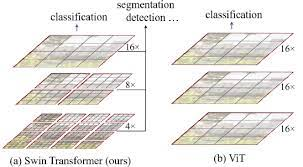
\includegraphics[width=9.5cm, height=5.5cm]{images/swin vs vit.png}
\centering
\caption{The difference between Swin Transformer and ViT \protect\cite{swin-v1}}
\label{fig:swin-vs-vit}
\end{figure}

Swin Transformer is made up of 4 stages as shown in \ref{fig:swin architecture1}. The input image has a dimension of H x W x 3. Swin Transformer uses a patch size of 4x4 which will produce H/4 x W/4 number of patches, and each patch’s feature dimension is 48 (4 x 4 x 3). In stage 1, the linear layer projects the raw-valued features to an arbitrary dimension $C$.

In stage 2, the patch merging layer concatenates the features of each group of 2 x 2 neighboring patches. Each patch’s feature dimension becomes 4C, on which it applies a linear layer, reducing the output dimension to 2C. So, we have H/8 x W/8 patches, each of which has 2C-dimensional features. The same processes are repeated in stages 3 and 4, reducing the size by 4 and increasing the feature dimension by 2.

\FloatBarrier
\begin{figure}[ht]
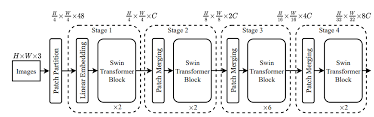
\includegraphics[width=11.5cm, height=4.5cm]{images/swin-transformer-4block.png}
\centering
\caption{Swin Transformer V1 Architecture \protect\cite{swin-v1}}
\label{fig:swin architecture1}
\end{figure}

The self-attention modeule in ViT has $O(n^2) $computational complexity to the number of tokens which makes it unsuitable forsemantic segmentation which require dense high-resolution classifications. Swin Transformer introduced a Shifted Window Multi-headed Self-Attention (W-MSA) to make the self-attetion linear to the number of tokens. The computational complexity of the original Multi-Headed Self-Attention is:
\begin{equation}
    \Omega (\mathbf{MSA}) = 4hwC^2 + 2(hw)^2C
\end{equation}
Where $h$ is the height of the patch, $w$ is the width of the patch and $C$ is the feature size. While the improved computational complexityof W-MSA is linear to the number of patches as shown in the equation below:
\begin{equation}
    \Omega (\mathbf{W-MSA}) = 4hwC^2 + 2M^2hwC
\end{equation}

Swin Transformer alternates between two partitioning configurations in consecutive Swin Transformer blocks. As shown figure \ref{fig:swin shifted}, layer 1 uses regular partitioning while layer 2 uses a windowing configuration shifted by half of the window size. They introduces connections between neighboring windows while keeping the local computation within each non-overlapping window.

The main issue with this approach is the number of local windows increased from 4 to 9. For this reason, Swin Transformer uses another mechanism called cyclic shifting. Cyclic shifting shift the image patches toward the top-left direction and then applies a masking mechanism to limit self-attention within adjacent patches. It also utilizes reverse cyclic shifting to cover the other areas. Cyclic shifting is shown in figure \ref{fig:swin cyclic}
\begin{figure}[ht]
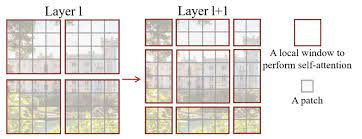
\includegraphics[width=10.5cm, height=4.5cm]{images/swin-msa1.jpeg}
\centering
\caption{Shifted Window Multi-head Self-Attention \protect\cite{swin-v1}}
\label{fig:swin shifted}
\end{figure}

\begin{figure}[ht]
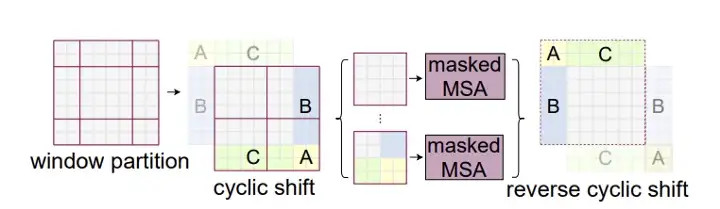
\includegraphics[width=13.5cm, height=5.5cm]{images/swin-cyclic-shift.jpg}
\centering
\caption{Cyclic Shifted Windows in Swin Transformer \protect\cite{swin-v1}}
\label{fig:swin cyclic}
\end{figure}

SW-MSA successfully introduced connections between windows while masking prevents the attention computation from processing across the image boundary. Figure \ref{fig:2swins} show two consecutiveSwin Transformer blocks with each one having a different partitioning scheme.
\FloatBarrier
\begin{figure}[ht]
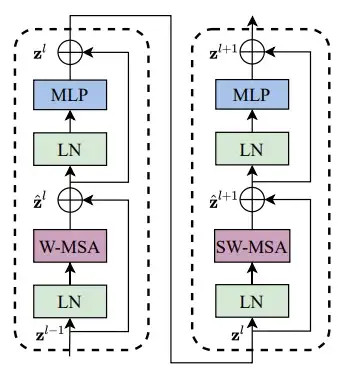
\includegraphics[width=6.5cm, height=7cm]{images/swin-architecture.jpg}
\centering
\caption{Two Successive Swin Transformer Blocks \protect\cite{swin-v1}}
\label{fig:2swins}
\end{figure}

The self-attention score using SW-MSA can be calculated as follows:
\begin{equation}
    Attention(Q,K,V) = softmax(\frac{QK^T}{\sqrt{d}+B})V
\end{equation}

Swin Transformer V2 \cite{swin-v2} was introsuced in 2021 and it is an improved version of Swin Transformer to increase scability, accuracy and stablity during training. As shown in figure \ref{fig:swin v1 vs v2}, the Layer Normalization block is moved from front to back of the residual unit and a new scaled cosine self-attention unit is used inplace of the old matrix multiplication based self-attention. The new self-attention score can be calculated as:
\begin{equation}
    Sim(\mathbf{q}_i,\mathbf{k}_j) = \frac{cos(\mathbf{q}_i,\mathbf{k}_j)}{\tau} + B_{ij}
\end{equation}

Where $B_{ij}$ is the relative position bias between pixel i and j; $\tau$ is a learnable scalar, non-shared across heads and layers.$\tau$ is set larger than 0.01. These approaches make the model insensitive to the magnitude (largeness) of activations.
\FloatBarrier
\begin{figure}[ht]
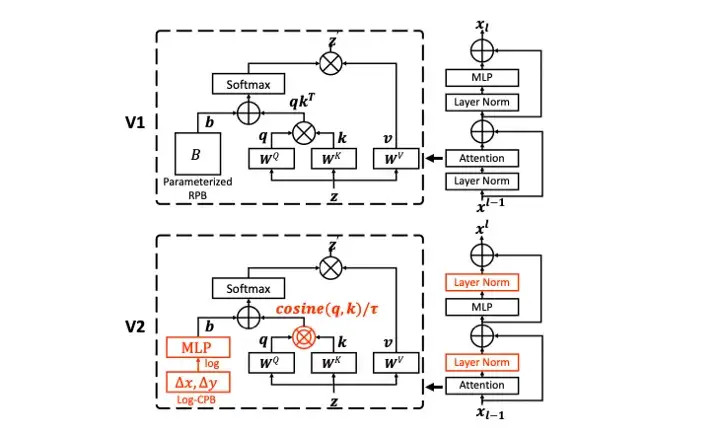
\includegraphics[width=13.5cm, height=9.5cm]{images/swin1-vs-swin2.jpg}
\centering
\caption{Difference Between Swin V1 and Swin V2 \protect\cite{swin-v2}}
\label{fig:swin v1 vs v2}
\end{figure}
\FloatBarrier

\subsection{UNetFormer}
%%unetformer
UNetFormer \cite{unetformer} proposes a UNet-like Transformer for semantic segmentation task trained using the UAVid, Vaihingen, Potsdam and LoveDA datasets.UNetFormer has the same encoder-decoder framework as the other U-Net variants. Referring to figure \ref{fig:unetformer} UNetFormer uses pretrained ResNet18 as its encoder and a Transformer with an added global-local Transformer block (GLTB) that are used as its decoder. 

ResNet18 consists of four stages and each stage will down-sample the feature map with a scale factor of 2. The feature maps generated by each stage are fused with the corresponding feature maps of the decoder using a 1x1 convolution with the channel dimension of 64. The semantic features produced by the ResNet18 are aggregated with the features generated by the GLTB of the decoder using a weighted sum operation. 

\FloatBarrier
\begin{figure}[ht]
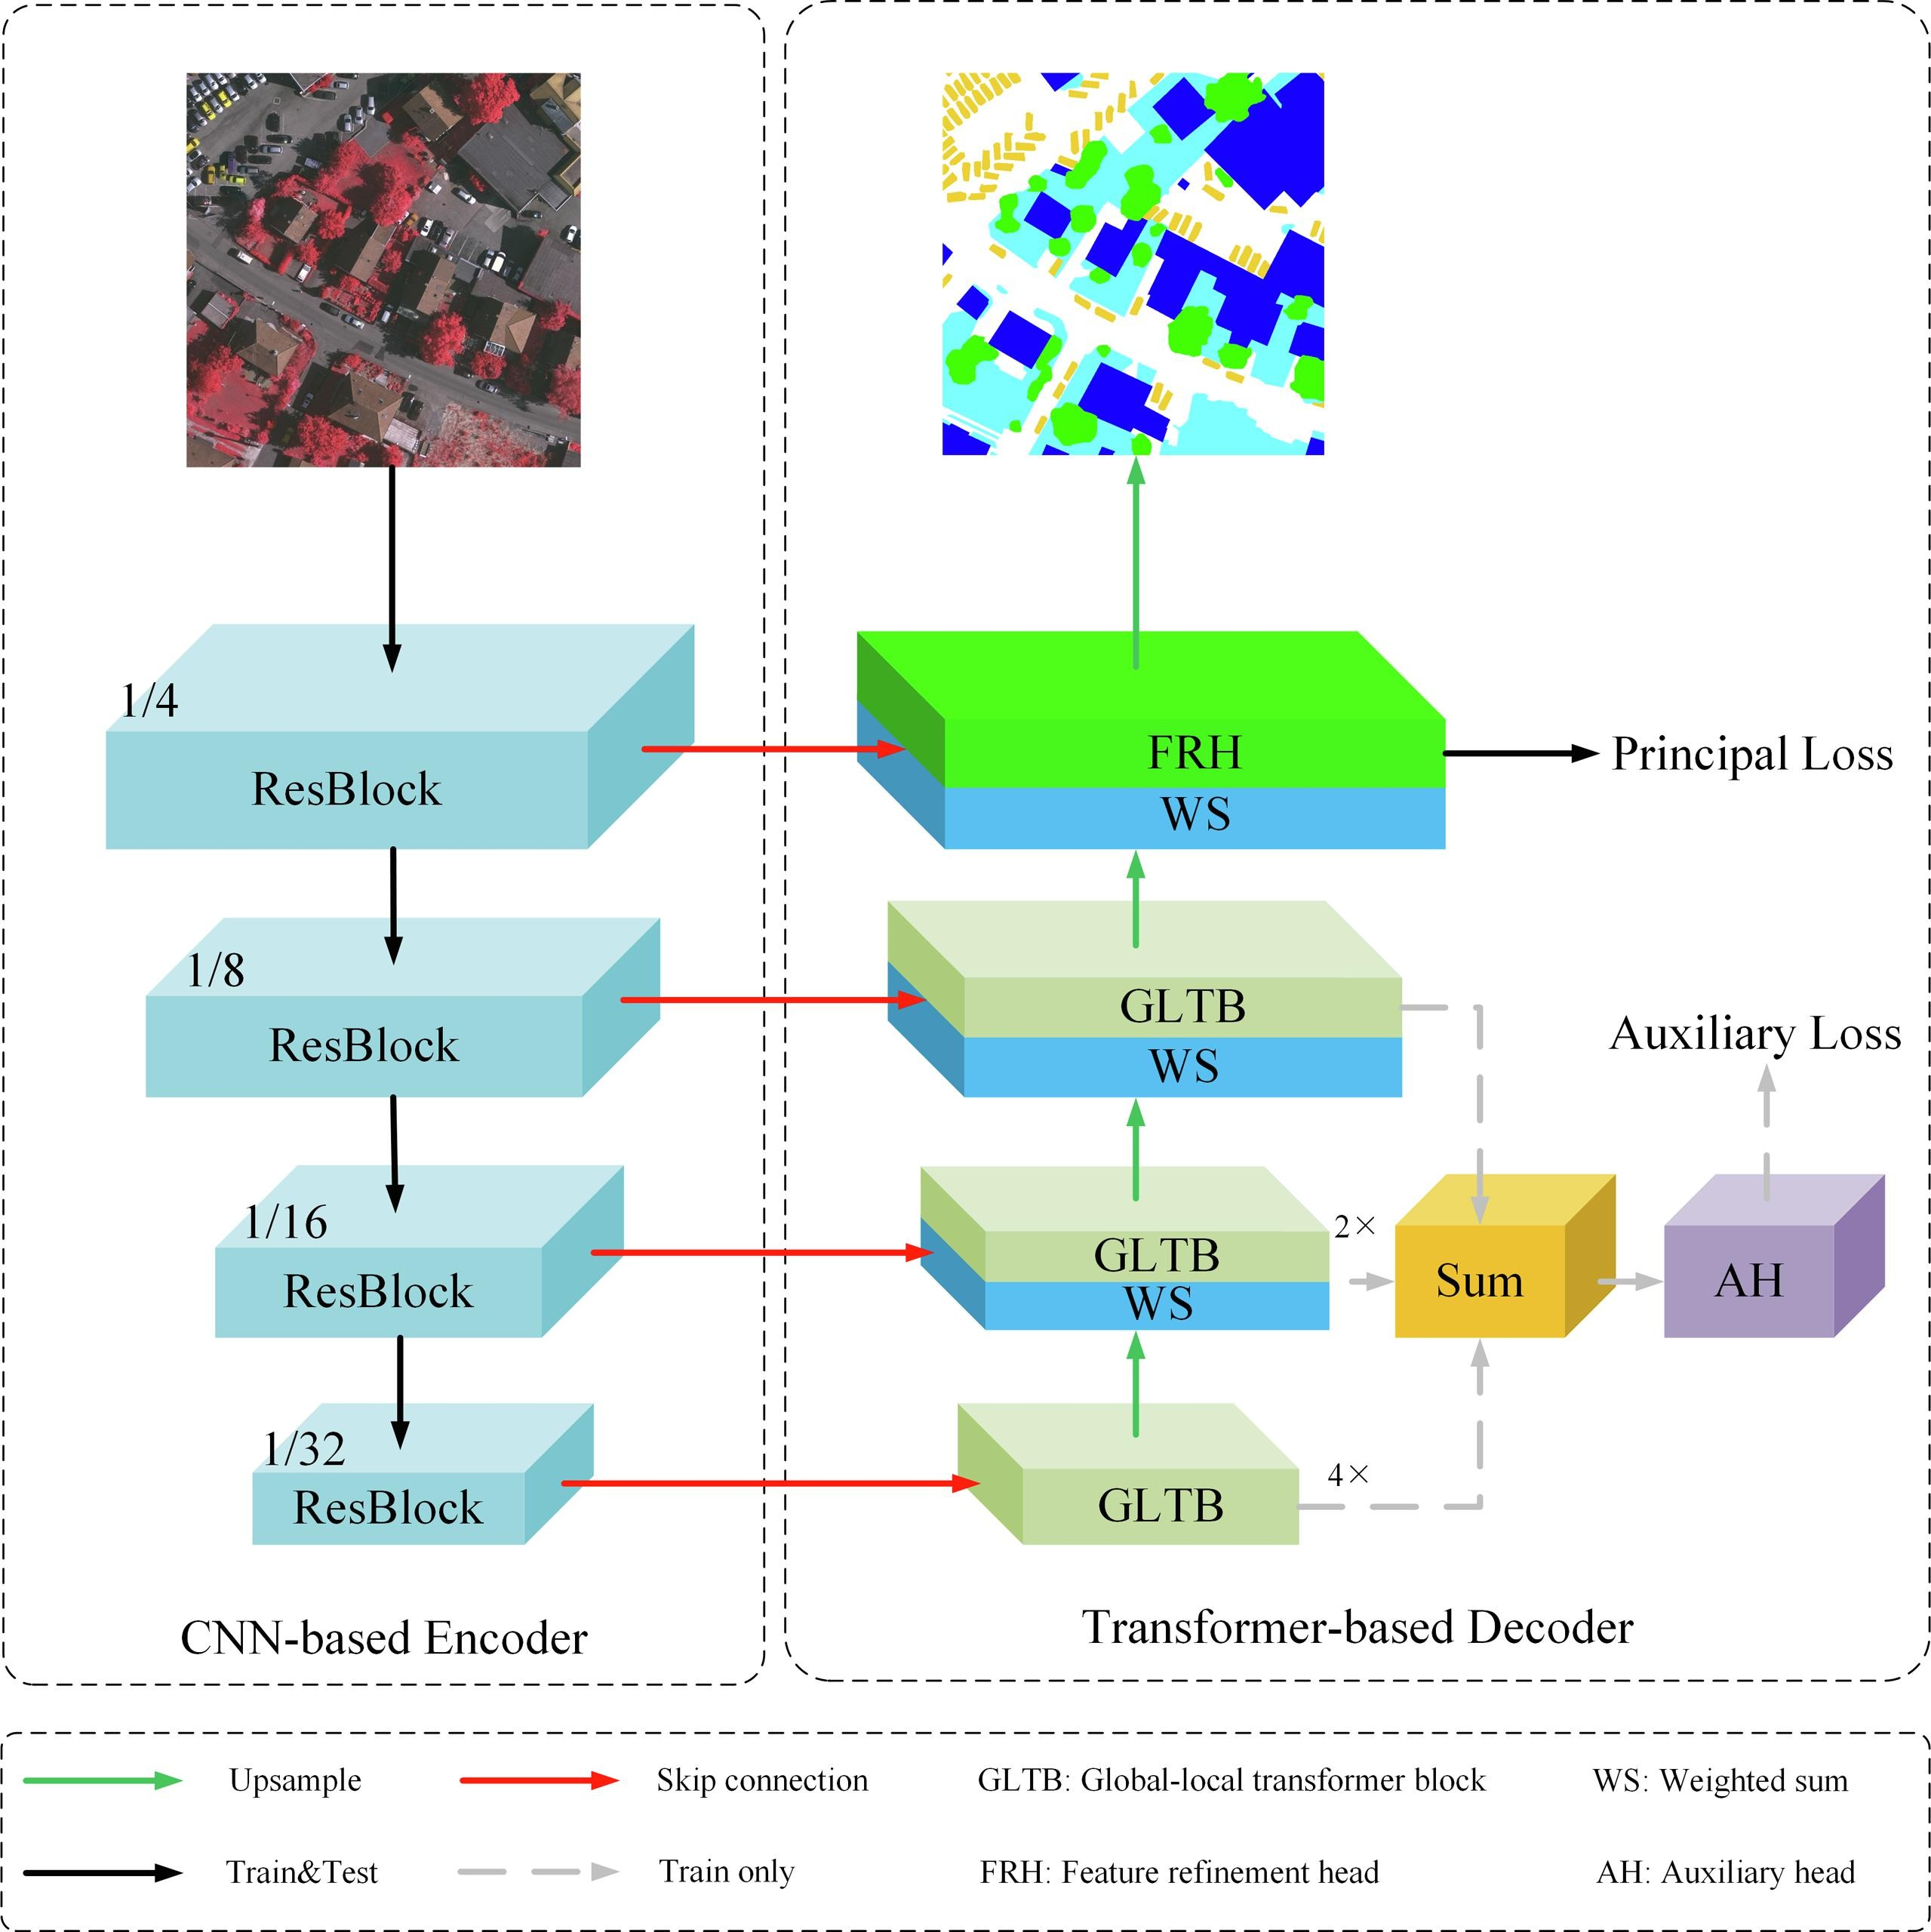
\includegraphics[width=10.5cm, height=7cm]{images/unetformer.jpg}
\centering
\caption{UNetFormer Architecture \protect\cite{unetformer}}
\label{fig:unetformer}
\end{figure}
\begin{figure}[ht]
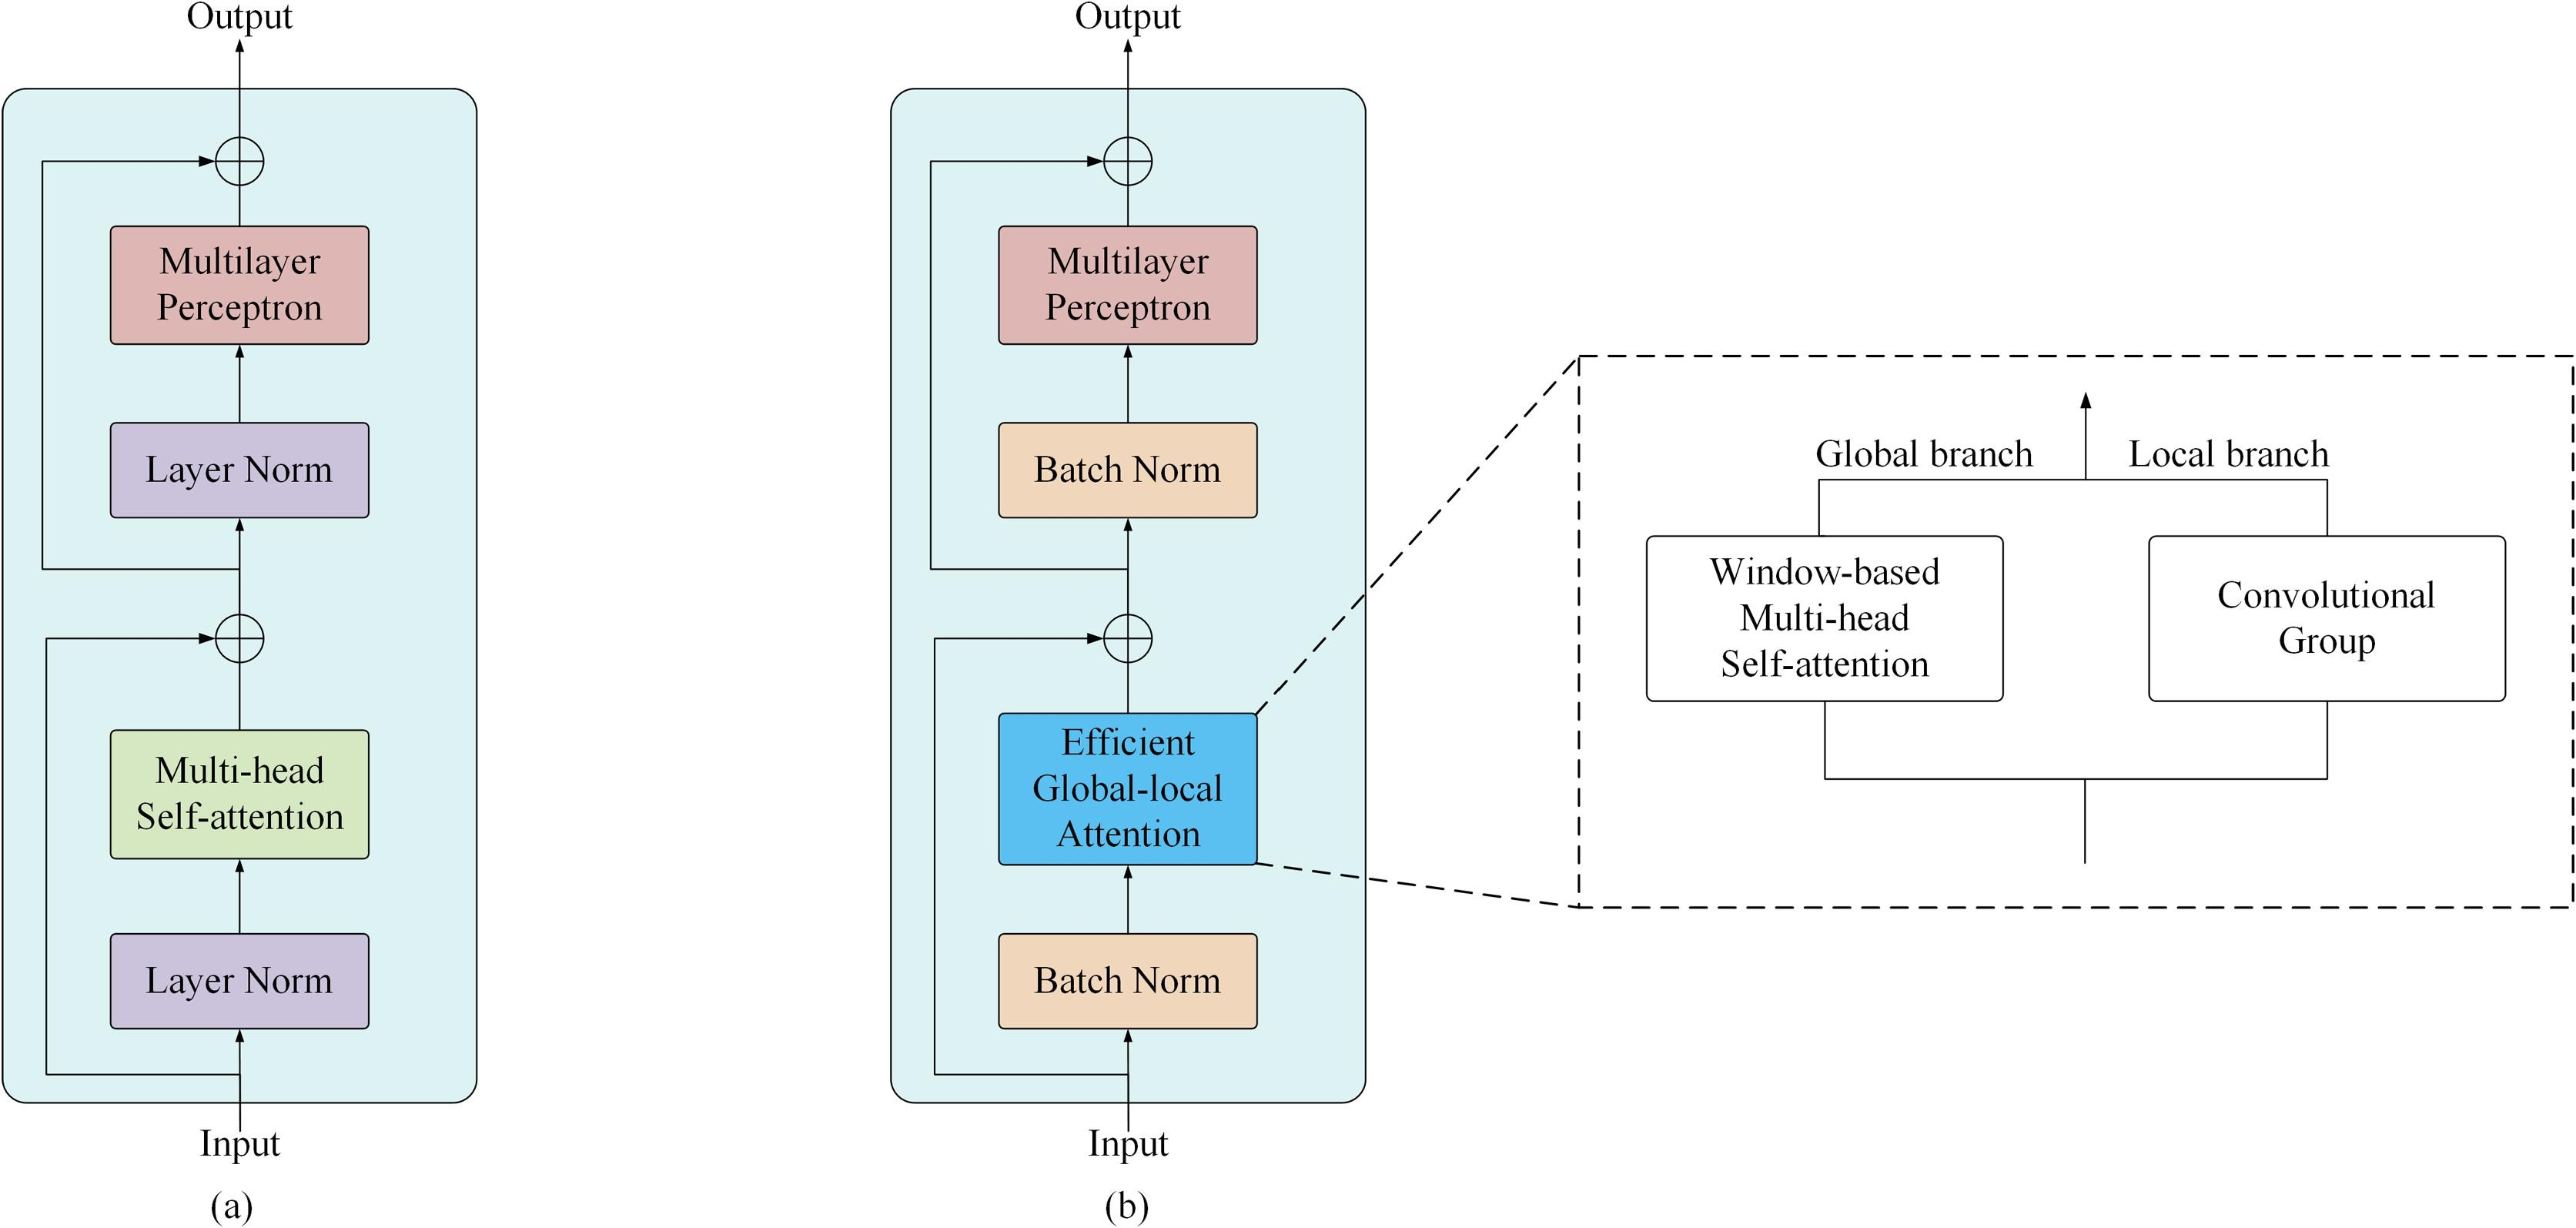
\includegraphics[width=10.5cm, height=7cm]{images/gltb.jpg}
\centering
\caption{ Illustration of (a) the standard Transformer block and (b) the Transformer block with GLTB \protect\cite{unetformer}}
\label{fig:gltb}
\end{figure}

The GLTB is made up of the global–local attention, multilayer perceptron, two batch normalization layers and two additional operations. The global–local attention has two  branches, the local branch and the global branch as shown in figure \ref{fig:unetformer-besar}. The local branch uses two parallel convolutional layers with kernel sizes of 3 and 1 to extract the local context. Two batch normalization operations are employed before the final sum operation.As illustrated in figure \ref{fig:unetformer-besar} the global btanch uses the same window-based multi-head self-attention in Swin Transformer to capture the global context.
\FloatBarrier
\begin{figure}[ht]
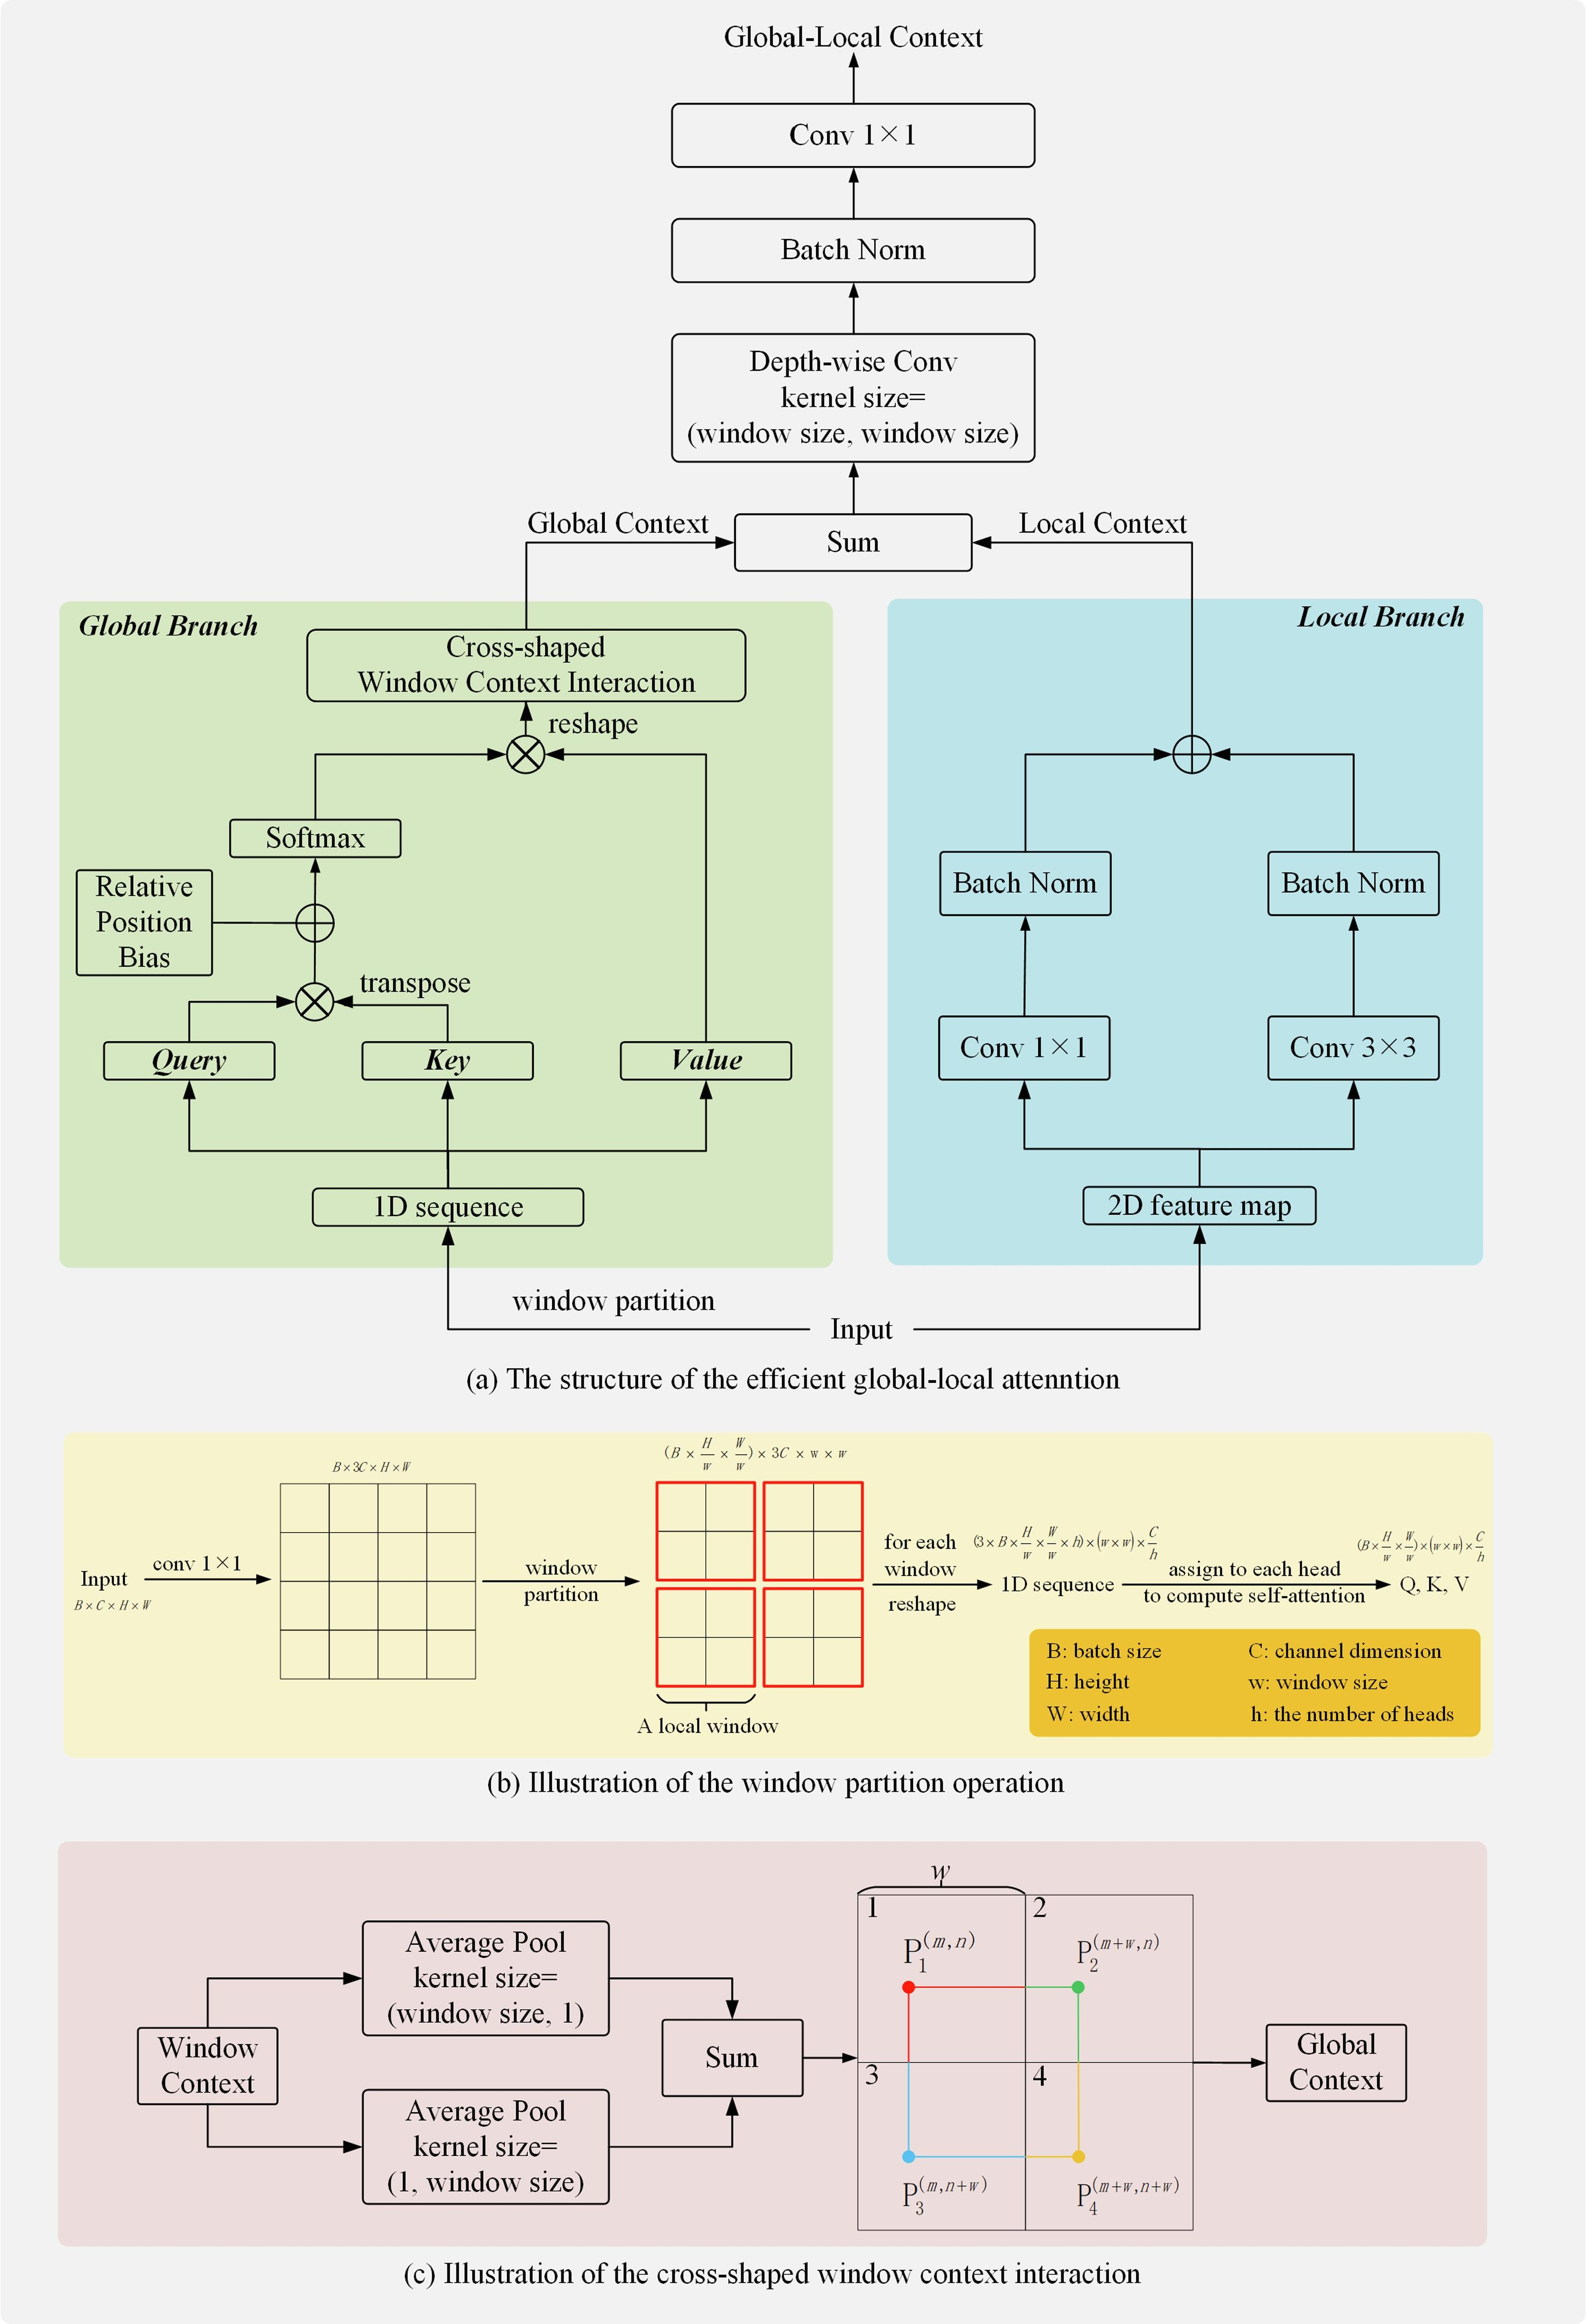
\includegraphics[width=13.5cm, height=18cm]{images/unetformer besar.jpg}
\centering
\caption{Cross-shaped Window Context Interaction in UNetFormer \protect\cite{unetformer}}
\label{fig:unetformer-besar}
\end{figure}
\FloatBarrier

The Swin Transformer uses a shifting windows mechanism to generate the relationship between the windows but this significantly increases the computation thus the author proposed  a cross-shaped window context interaction to reduce the computation. The cross-shaped window context interaction captures the global context by fusing the two feature maps produced by a horizontal average pooling layer and a vertical average pooling layer. The horizontal average pool layer generates the horizontal relationship between windows, such as $Win_1 = H(Win_2)$. For any point $P^{m,n}_1$ win $Win_1$ its dependency with $P^{m+w,n}_2$ can be expressed as:

\begin{equation}
    P^{m,n}_1 = \frac{\sum^{w-m-1}_{i=0}P^{m+i,n}_1 + \sum^m_{j=0}P^{m+w-j,n}_2}{w}
\end{equation}
\begin{equation}
    P^{m+i,n}_1 = D_i (P^{m,n}_1)
\end{equation}
\begin{equation}
    P^{m+w-j,n}_2 = D_j(P^{m+w,n}_2)
\end{equation}

\FloatBarrier
Where w is the window size and D denotes the self-attention computation. Similarly, the vertical relationship between $Win_1$ and $Win_3$ can be established in a similar way, $Win_1 = V(Win_3)$ and for $Win_4$ the realtionship is $Win_1 = V(H(Win_4)) + H(V(Win_4))$. 

\FloatBarrier

\begin{figure}[ht]
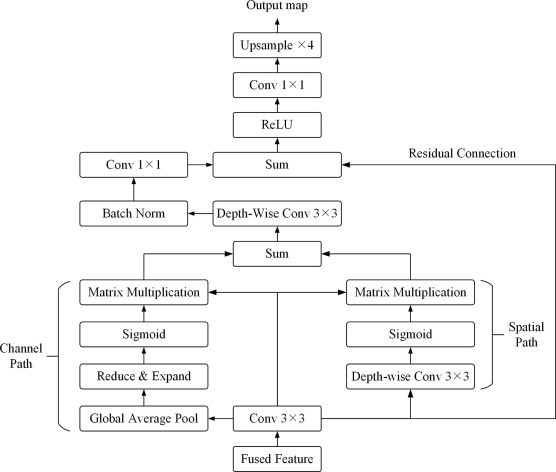
\includegraphics[width=10.5cm, height=7cm]{images/frh.jpg}
\centering
\caption{Feature refinement Head of UNetFormer \protect\cite{unetformer}}
\label{fig:frh}
\end{figure}

\FloatBarrier

Finally, UNetFormer uses a Feature Refinement Head (FRH) just before the output is produced. The reason why FRH is needed is because while the ResNet encoder provides rich spatial details of satellite images, it lacks semantic content, on the other hand the deep GLTB provides precise semantic information, but with a coarse spatial resolution. FRH shrinks the semantic gap between the two features for improved accuracy. FRH received the fused feature as shown in \ref{fig:unetformer} as its input. Then, two path are constructed to strengthen the channel-wise and spatial-wise feature representation as shown in figure \ref{fig:frh}. The first path is called the channel path while the second path is called the spatial path. The channel path employs a global average pooling layer to generate a channel-wise attentional map $\textbf{C} \in \mathbb{R}^{1\times 1 \times c}$ , where c is the channel dimension. The reduce \& expand operation contains two 1 x 1 convolutional layers, which first reduces the channel dimension c by a factor of 4 and then expands it to the original dimension. The spatial path utilizes a depth-wise convolution to produce a spatial-wise attentional map $\textbf{S} \in \mathbb{R}^{h\times w \times 1}$  , where h and w are the height and width of the feature map. The features generated by the two paths are fused before a 1x1 convolutional layer and an upsampling operation are applied as post processing.

%%%LANET%%%%%%
\subsection{LANet}
Local Attention Network (LANet) \cite{lanet}introduced two additional modules to improve semantic segmentation of satellite images. The first module is the Patch Attention Module (PAM) to enhance the embedding of local context information. The second module is the Attention Embedding Module (AEM) to improve the use of spatial information. Referring to figure \ref{fig:lanet} The high-level features produced by late layers of CNNs will pass through a PAM to enhance its feature, while the low-level features produced by early layers of a CNN are first enhanced by a PAM, before being embedded with semantic information from high-level features through AEM. The final ouput is the fusion of the outputs from the top and bottom channels. 

\FloatBarrier
\begin{figure}[ht]
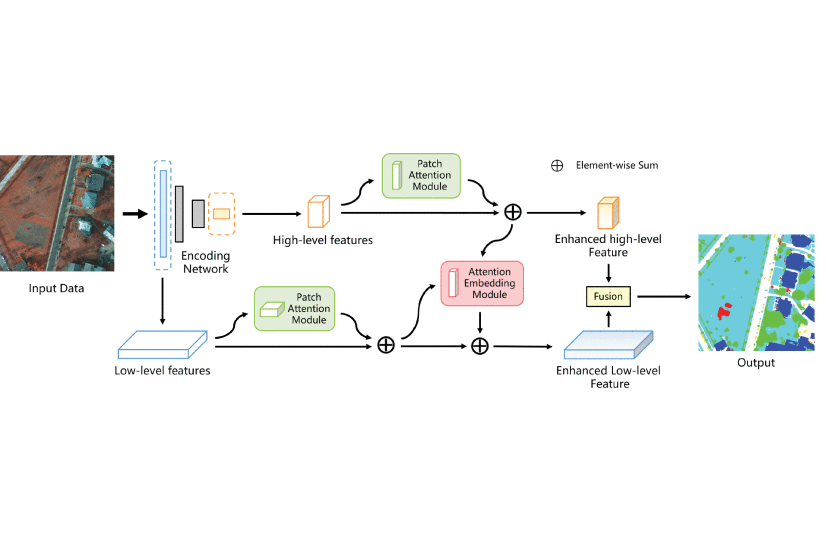
\includegraphics[width=12.5cm, height=9.5cm]{images/lanet.png}
\centering
\caption{LANet Architecture \protect\cite{lanet}}
\label{fig:lanet}
\end{figure}

\FloatBarrier

Referring to figure \ref{fig:pam}, PAM will first generate a local descriptor for each channel of every patch. The descriptor $z_c$ for the $c$ th channel of a patch is calculated as

\begin{equation}
    z_c = \frac{1}{h_p w_p} \sum_{i=1}^{h_p} \sum_{j=1}^{w_p} x_c(i,j)
\end{equation}

where $h_p$ and $w_p$ is the horizontal and vertical size of the patch and $x_c$ is the pixel value at the $c$ th channel. In this way, a c-channel vector $z_p$ will be generated, which contains the statistics describing the patch p. Then, they apply convolutional layer to learn an attention vector $a_p \in \mathbb{R}^{c \times h_p \times w_p}$. The entire gating operation to generate attention maps includes a 1 x 1 dimension-reduction convolution, 1×1 dimension-increasing convolution that recovers the feature dimension back to $c$ and an upsampling operation.
\begin{figure}[ht]
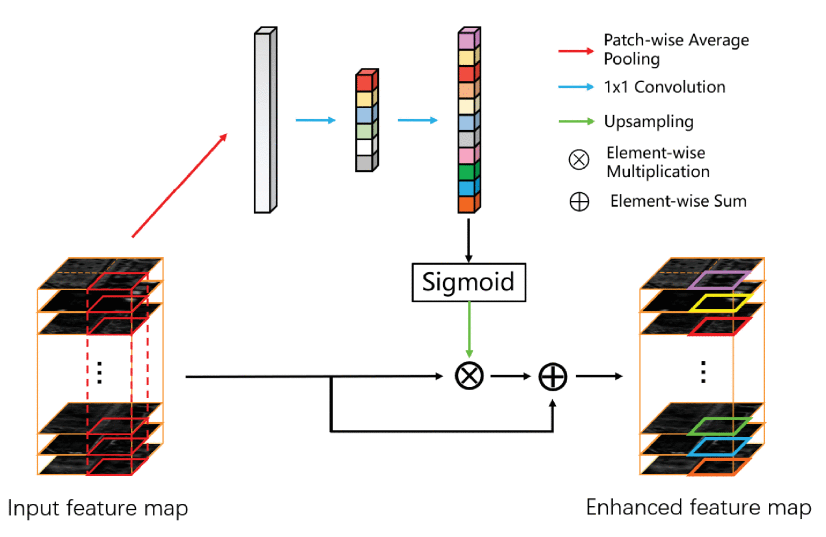
\includegraphics[width=9.5cm, height=4.5cm]{images/pam.png}
\centering
\caption{Patch Attention Module in LANet \protect\cite{lanet}}
\label{fig:pam}
\end{figure}
\FloatBarrier

In most networks, the most frequently used way of employing low-level features is to concatenate them with high-level features, which brings only slight improvement in performance. The authors proposed AEM to bridge the gap between high-level and low-level features without sacrificing the spatial details of the latter. Figure \ref{fig:aem} shows the implementation of AEM. First, they generate a high-level feature descriptor map, $z_c$ and low-level descriptor map , $x_c$ usinging the same formula in PAM. Then, an attention map, $a_c$ is generated using average pooling, 1 x 1 convolution and upsampling. Finally $a_c$ will be added to $x_c$ to generate an improved low-level descriptor.  
\begin{figure}[ht]
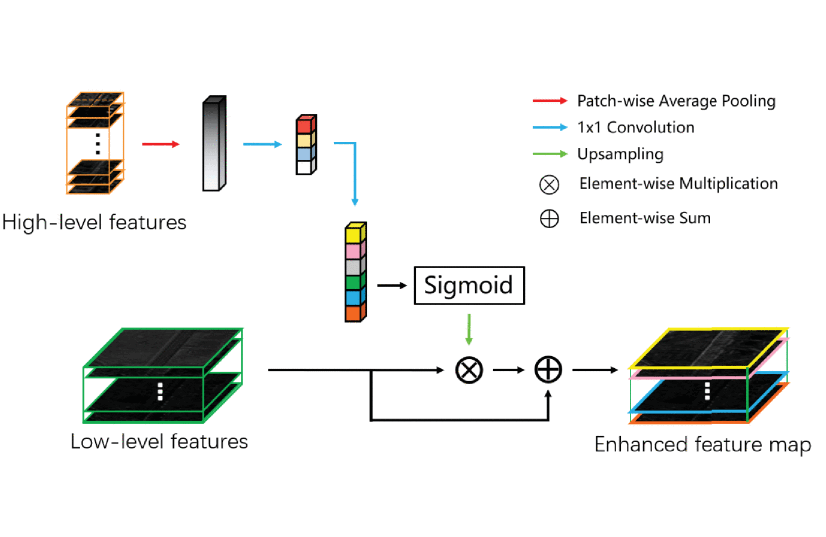
\includegraphics[width=9.5cm, height=4.5cm]{images/aem.png}
\centering
\caption{Attention Embedding Module in LANet \protect\cite{lanet}}
\label{fig:aem}
\end{figure}
\FloatBarrier


%%%%%%%A Novel Transformer Based Semantic Segmentation Scheme for Fine-Resolution
\subsection{DC-Swin}
A novel semantic segmentation scheme of densely connected (DC-Swin) \cite{a-novel-transformer} proposed by combining Swin Transformer and a densely connected feature aggregation module (DCFAM). Swin Transformer is used as the encoder to extract the context information while DFCAM act as the decoder to restore the resolution and produce the segmentation map.

\FloatBarrier
\begin{figure}[ht]
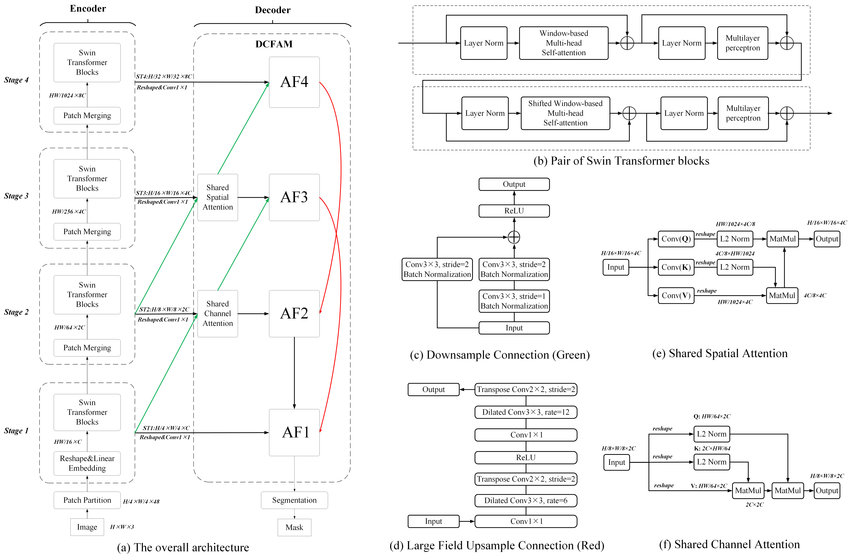
\includegraphics[width=12.5cm, height=6.5cm]{images/dc-swin.png}
\centering
\caption{(a) Overall architecture of DC-Swin. (b) Pair of Swin Transformer blocks. (c) Downsample Connection. (d) Large Field Upsample Connection. (e) SSA. (f) SCA \protect\cite{a-novel-transformer}}
\label{fig:dc}
\end{figure}

Referring to figure \ref{fig:dc}(a), the Swin Transformer split the input RGB image into nonoverlapping patches as "tokens" using a patch partition module. This tokens are then fed into the multistage feature transformation. In stage 1, a linear embedding layer is deployed to project features to an arbitrary dimension $C$. Next, a pair of Swin Transformer as shown in figure \ref{fig:dc}(b) are utilized to extract semantic features. In stages 2 to 4, the number of tokens is gradually reduced by patch merging layers along with the increasing depth of the network to produce a hierarchical representation. The outputs of the four stages are processed by a standard 1 $\time$ 1 convolution to generate four hierarchical Swin Transformer features. By adjusting the hyperparameters of tge Swin Transformer, they can construct backbones with different complexities.

DFCAM has two important modules namely the Shared Spatial Attention (SSA) and a Shared Channel Attention (SCA) to enhance the spatial-wise and channel-wise relationship. Then, multi-level features are further integrated using the Downsample Connection and the Largefield Upsample Connection for improving m lti-scale. According to figure \ref{fig:dc} DFCAM connects the four hierarchical features with cross-scale connections and attention blocks to generate four aggregation features: AF1, AF2, AF3, and AF4.  

The Downsample connection which is the green line in figure \ref{fig:dc} connects the low-level and high-level transformer features for fusion and it can be defined as follow:
\begin{equation}
    D^i_j(\mathbf{X}) = f_\sigma(f_\delta(\mathbf{X}) + f_\mu(f_\theta(\mathbf{X})))
\end{equation}

Where $\mathbf{X}$ is the input vector; $f_\sigma$ is a ReLU activation function; $f_\delta$ and $f_mu$ are a 3x3 convolution layer with a stride of 2; $f_\theta$ is a 3x3 convolution layer with astride of 1 with each convolution layer involves a batch normalization operation; $i$ and $j$ are the number of the input channels and output channels.

The red line is the Large field Upsample Connection. It is used to capture multi-scale
context effectively and can be mathematically expressed as:
\begin{equation}
    LU^n_m(\mathbf{X}) = f^{12}_\varphi(f_\sigma(f^6_\varphi(\mathbf{X})))
\end{equation}

Where $f^{12}_\varphi$ is a composite function that contains a standard 1x1 convolution, a dilated convolution with a dilated rate of 12, and a standard transpose convolution; $f^{6}_\varphidilated$ is similar but with a dilated rate of 6; $m $and $n$ are the number of the input channel and output channel.

SSA is used to model the long range dependencies and it is defined as: jangan fail
\begin{equation}
    SSA(\mathbf{X}) = \frac{\sum_n V(\mathbf{X}_{c,n})+\frac{Q(\mathbf{X})}{|||Q(\mathbf{X})||_2} ((\frac{K(\mathbf{X})}{||K(\mathbf{X}))||_2})^T V(\mathbf{X})}
    {N + \frac{Q(\mathbf{X})}{||Q(\mathbf{X})||_2} \sum_n(\frac{K(\mathbf{X})}{||K(\mathbf{X}))||_2})^T }
\end{equation}

Where $Q(\mathbf{X}), K(\mathbf{X})) and V(\mathbf{X}))$ are the convolutional operation to generate the Q, K and V; N is the number of pixels in the input feature maps; c is the channel dimension and n is the flattened spatial dimension.

SCA is used to extract the long-range dependencies between the channel dimensions and can be defined as:
\begin{equation}
    SCA(\mathbf{X}) = \frac{ R(\mathbf{X}_{c,n})+(R(\mathbf{X}_{c,n}))\frac{R(\mathbf{X})}{||R(\mathbf{X}))||_2})^T \frac{R(\mathbf{X})}{||R(\mathbf{X}))||_2} }
    {N + \frac{R(\mathbf{X})}{||R(\mathbf{X})||_2} \sum_c(\frac{R(\mathbf{X})}{||R(\mathbf{X}))||_2})^T }
\end{equation}

Where $R(\mathbf(X))$ is the reshape operation to flatten the spatial dimension.

Each of the aggregation features can be mathematically expressed as follows:
\begin{equation}
    \mathbf{AF_4} = \mathbf{ST_4} + D^{768}_{384} (SSA(D^{384}_{192}(\mathbf{ST_2}))
\end{equation}

\begin{equation}
    \mathbf{AF_3} = SSA(\mathbf{ST_3})+ D^{384}_{192} (SSA(D^{192}_{96}(\mathbf{ST_1}))
\end{equation}

\begin{equation}
    \mathbf{AF_2} = SCA(\mathbf{ST_2})+ LU^{192}_{768} (\mathbf{AF_4})
\end{equation}

\begin{equation}
    \mathbf{AF_1} = \mathbf{ST_1} + U(\mathbf{AF_2}) + LU^{96}_{384}(\mathbf{AF_3})
\end{equation}
where $U$ is a bilinear interpolation upsample operation with a scale factor of 2; $\mathbf{ST_1}, \mathbf{ST_2}, \mathbf{ST_3} and \mathbf{ST_4}$ are the Swin Transformer features from its respective block.
%%%%%%%%%% BANET
\subsection{BANet}
The architecture of Bilateral Awareness Network (BANet) is shown in figure \ref{banet} and it is madeup of two paths: the dependency path and the texture path. The texture path is designed to extract textural feature and the dependency path is for capturing long range dependencies.

\FloatBarrier
\begin{figure}[ht]
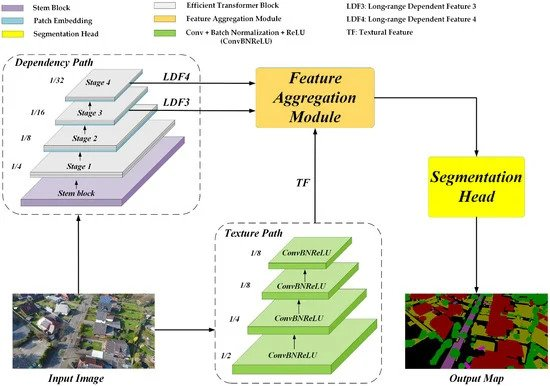
\includegraphics[width=12.5cm, height=6.5cm]{images/banet.jpg}
\centering
\caption{Architecture of Bilateral Awareness Network (BANet) \protect\cite{banet}}
\label{fig:banet}
\end{figure}

The dependency path is made up of a stem block and four Transformer stages to extract where each stage consists of two efficient transformer blocks (ETB). Stage 2,3 and 4 has a patch embedding (PE) operation. The dependency pathwill generate two long range dependent features namely the LDF3 and LDF4. The ETB is made up of ResT-Lite \cite{restlite} pretrained on ImageNet. ETB as illustrated in figure \ref{fig:etb} uses efficient multihead self-attention (EMSA) instead of the usual multi-headed self attention.

\FloatBarrier
\begin{figure}[ht]
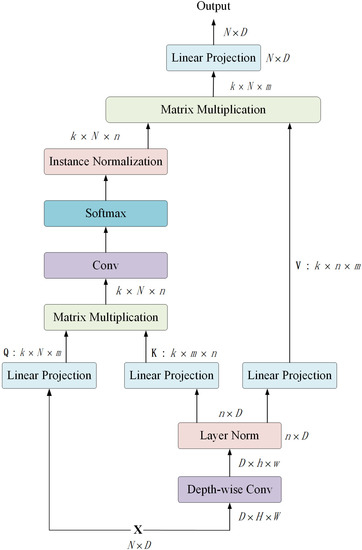
\includegraphics[width=4.5cm, height=7.5cm]{images/etb.png}
\centering
\caption{Efficient Transformer Block \protect\cite{banet}}
\label{fig:etb}
\end{figure}

The self-attention score from EMSA can be calculated as follows:
\begin{equation}
    EMSA(\mathbf{Q,K,V}) = LP(IN(softmax(conv(\frac{\mathbf{QK}^T}{\sqrt{m}}))).\mathbf{V})
\end{equation}
where IN is the instance normalization function and LP stands for linear projection.

The texture path has four convolution layers and each convolutional layer is equipped with batch normalization and ReLU activation function. The downsampling factor is set to 8. The output for the texture path can be expressed as:
\begin{equation}
    TF(\mathbf{X}) = T_4(T_3(T_2(T_1(\mathbf{X}))))
\end{equation}
where each T represents a combined function consisting of a convolutional layer, a batch
normalization operation, and a ReLU activation function. The convolutional layer in $T_1$ has a
kernel size of 7 and a stride of 2, which expands the channel dimension from 3 to 64. For
$T_2$ and $T_3$, the kernel size and stride are 3 and 2, respectively. The channel dimension is
kept as 64. Lastly for $T_4$, the convolutional layer is a standard 1x1 convolution with a stride of 1, expanding the channel dimension from 64 to 128. Thus, the output textural feature is
downscaled 8 times and has a channel dimension of 128.

The last module in BANet is the Feature Aggregation Module (FAM) and it is designed to leverage the benefits of the dependent features and texture features for powerful feature representation. FAM is illustrated in figure \ref{fig:fam}. The input features for the FAM include the LDF3, LDF4 and TF. To fuse those features, they first employ an attentional embedding module (AEM) to merge LDF3 and LDF4. Then, the merged feature is upsampled to concatenate with the TF to produce the aggregated feature. Finally, the linear attention module is deployed to reduce the fitting residual of the aggregated feature.

\FloatBarrier
\begin{figure}[ht]
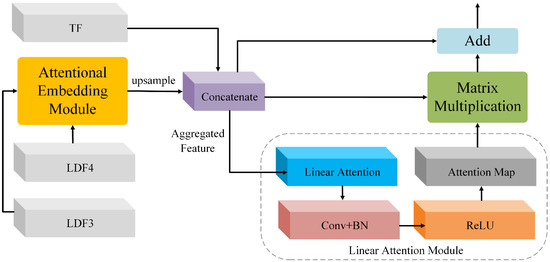
\includegraphics[width=7.5cm, height=5.5cm]{images/fam.jpg}
\centering
\caption{Feature Aggregation Module \protect\cite{banet}}
\label{fig:fam}
\end{figure}

%%%%%%unet-transformer
\subsection{AESwin-UNet}
Adaptive Enhanced Swin Transformer with U-Net (AESwin-UNet) \cite{unet-transformer}  uses a combination of Vision Transformer and U-Net for semantic segmentation of satellite images. As shown in figure \ref{fig:unetswin} instead of using CNN for the encoder, they opted to use Enhanced Swin Transformer instead.  For the decoder, each step involves an up-sampling of the feature map followed by a 2 × 2 deconvolution, a concatenation with a feature map from the encoder, and two 3 × 3 convolutions. 

\FloatBarrier
\begin{figure}[ht]
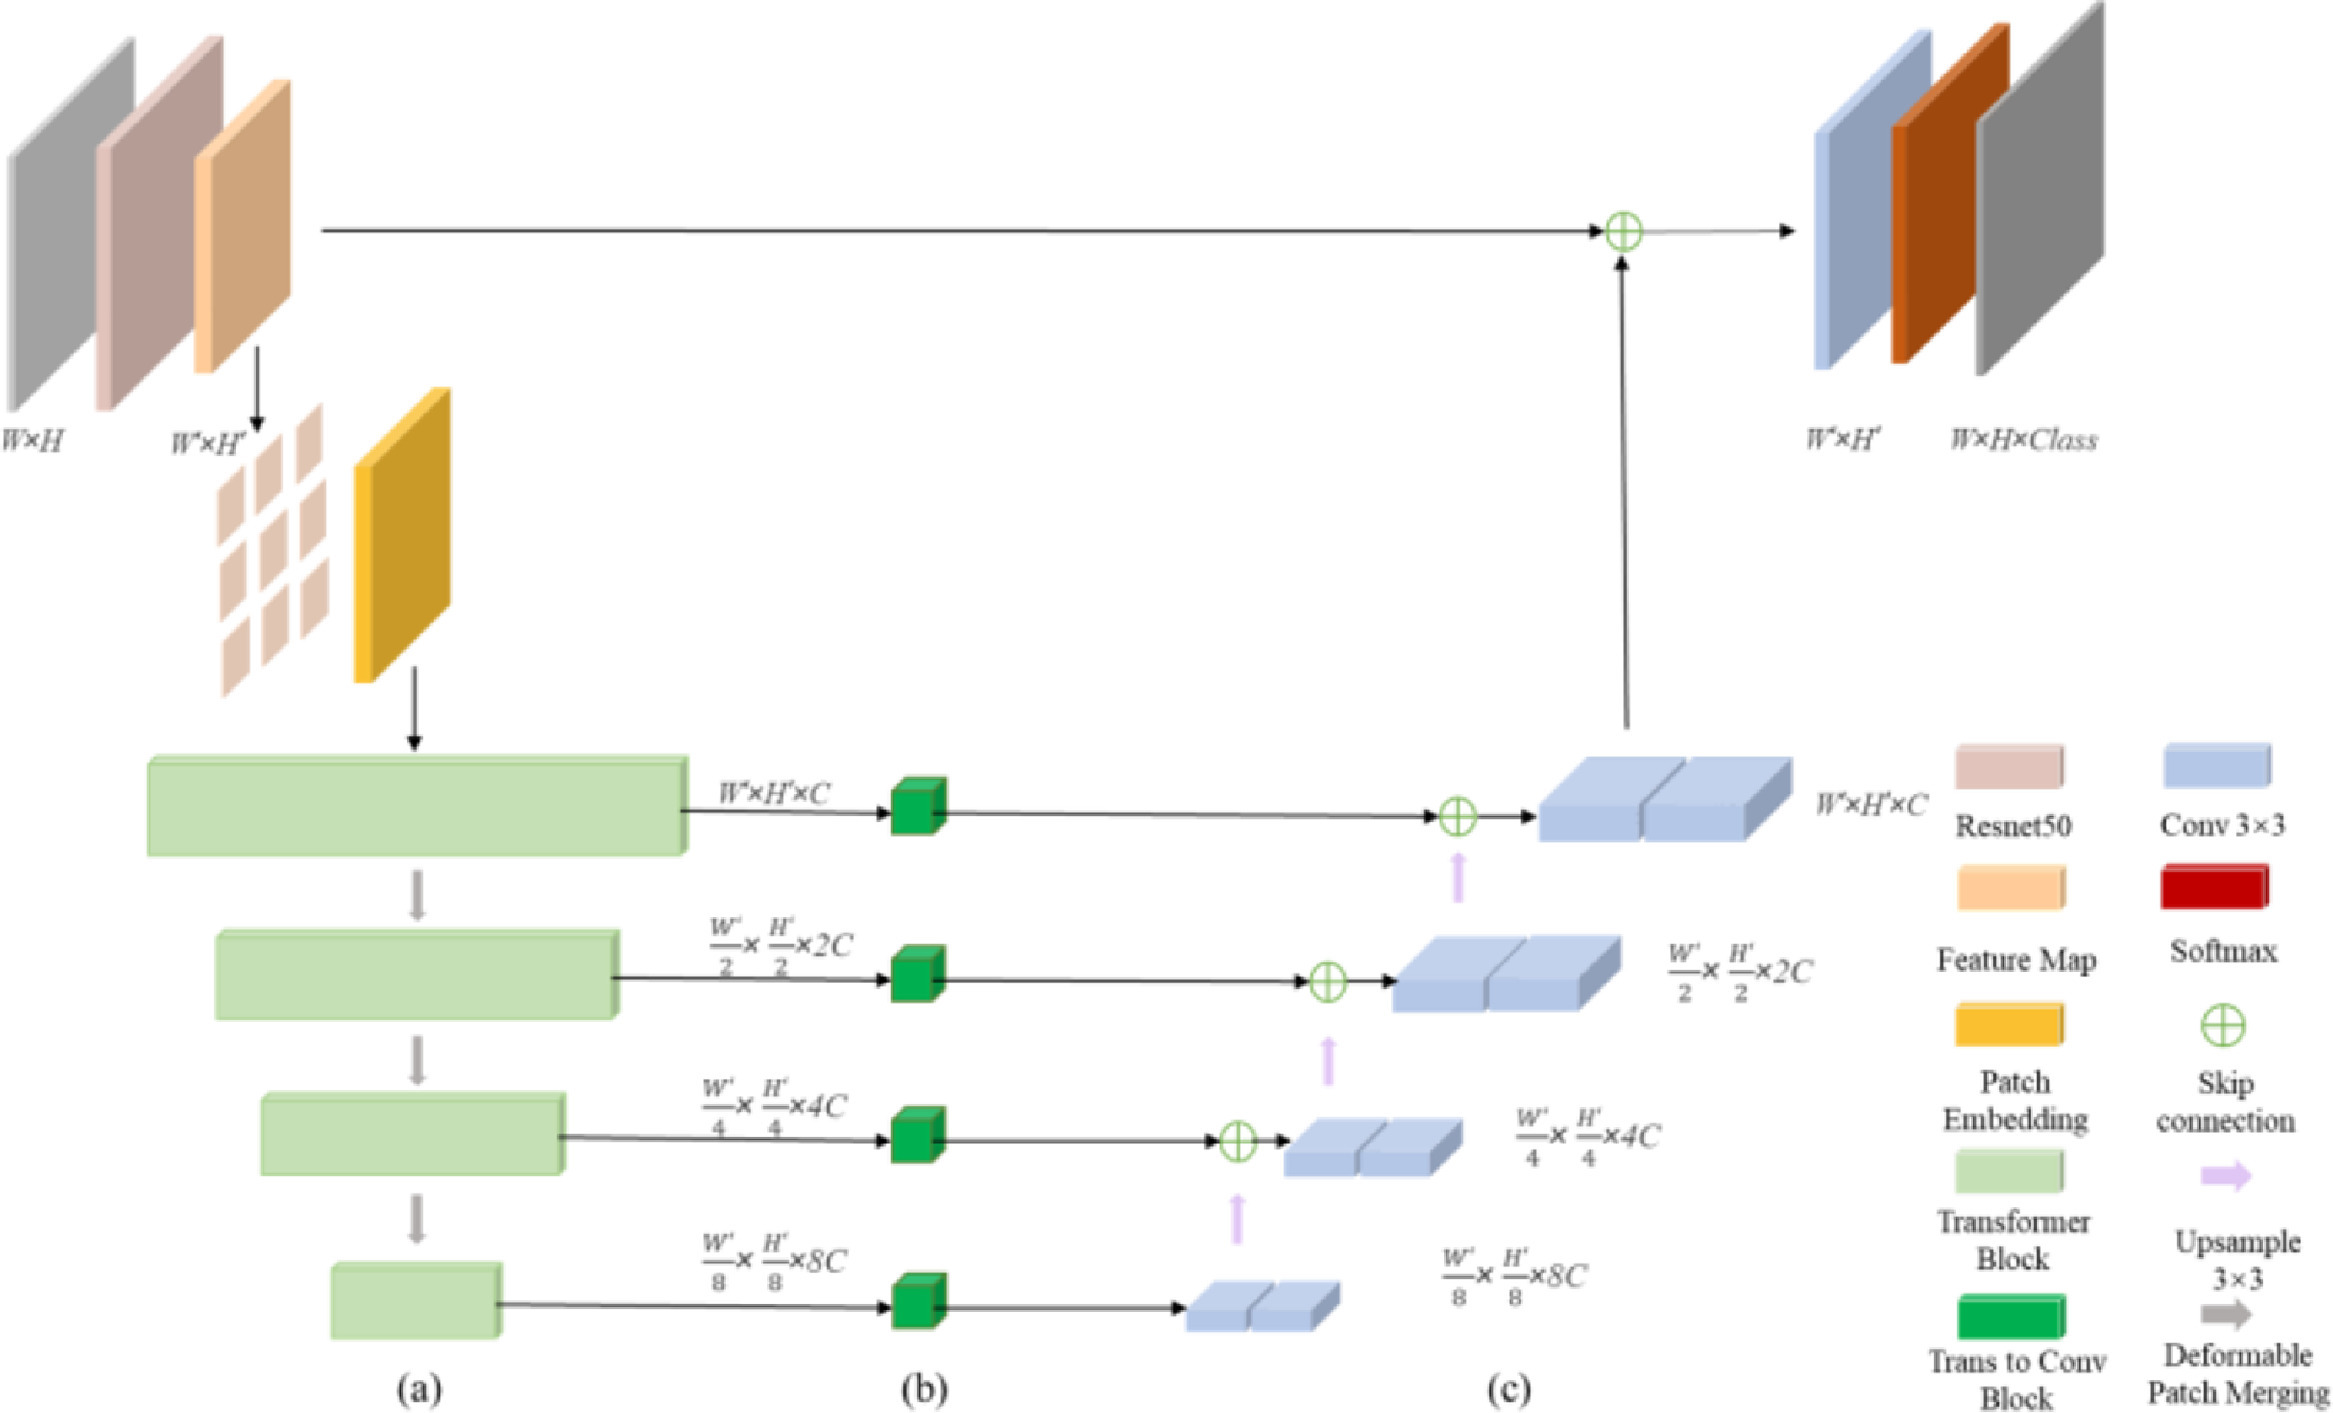
\includegraphics[width=12.5cm, height=8.5cm]{images/unet-trasnformer.jpg}
\centering
\caption{Architecture of Adaptive Enhanced Swin Transformer with U-Net (AESwin-UNet) \protect\cite{unet-transformer}}
\label{fig:unetswin}
\end{figure}

Enhanced Swin Transformer is a Swin Transformer  with enhanced multi-head self-attention (EMHSA) and deformable adaptive patch merging layer (DeforAPM). The EMHSA calculate  the attention score by fusing the low-level features and the global channel context. The enhanced attention can be formally defined as:

\begin{equation}
    Attention(Q,K,V) = Softmax(\fraction{att(QK^T)}{\sqrt{d_k}}+B)V
\end{equation}

\subsection{Summary of Semantic Segmentation Using Transformer}

The three tables below contain the F1-score, mIou score and accuracy score of each semantic segmentation model reviewed.

\FloatBarrier
\begin{table}\centering\setlength\tabcolsep{3.5pt}\renewcommand\arraystretch{1.25}
  \noindent\makebox[\textwidth]{%
    \begin{tabular}{|l|*{4}{c|}}
      \hline
      \diagbox[width=\dimexpr \textwidth/8+10\tabcolsep\relax, height=1cm]{ \textbf{Model} }{\textbf{Dataset}}
                   & \textbf{Potsdam} & \textbf{Vaihingen} & \textbf{LoveDA} & \textbf{UAVid}  \\
      \hline
        UNetFormer \cite{unetformer} & - & - & - & -\\
      \hline
        LANet \cite{lanet} & 91.95 & 88.09 & - & -\\
      \hline
        DC-Swin \cite{a-novel-transformer} & 93.25 & 90.71 & - & - \\
      \hline
        BANet \cite{transformer-meet-conv} & 92.50 & 89.58 & - & - \\
      \hline
        AESwin-Unet \cite{unet-transformer} & - & - & - & - \\
      \hline
    \end{tabular}
  }%
\caption{\label{tab:F1-score}F1-score achieved by each model.}

\end{table}

\begin{table}\centering\setlength\tabcolsep{3.5pt}\renewcommand\arraystretch{1.25}
  \noindent\makebox[\textwidth]{%
    \begin{tabular}{|l|*{4}{c|}}
      \hline
      \diagbox[width=\dimexpr \textwidth/8+10\tabcolsep\relax, height=1cm]{ \textbf{Model} }{\textbf{Dataset}}
                   & \textbf{Potsdam} & \textbf{Vaihingen} & \textbf{LoveDA} & \textbf{UAVid}  \\
      \hline
        UNetFormer \cite{unetformer} & 85.5 & 81.6 & - & 70\\
      \hline
        LANet \cite{lanet} & - & - & - & -\\
      \hline
        DC-Swin \cite{a-novel-transformer} & 87.56 & 83.22 & - & - \\
      \hline
        BANet \cite{transformer-meet-conv} & 86.25 & 81.35 & - & 64.6 \\
      \hline
        AESwin-Unet \cite{unet-transformer} & - & - & 66.1 & - \\
      \hline
    \end{tabular}
  }
\caption{\label{tab:miou}mIoU score achieved by each model.}

\end{table}

\begin{table}\centering\setlength\tabcolsep{3.5pt}\renewcommand\arraystretch{1.25}
  \noindent\makebox[\textwidth]{%
    \begin{tabular}{|l|*{4}{c|}}
      \hline
      \diagbox[width=\dimexpr \textwidth/8+10\tabcolsep\relax, height=1cm]{ \textbf{Model} }{\textbf{Dataset}}
                   & \textbf{Potsdam} & \textbf{Vaihingen} & \textbf{LoveDA} & \textbf{UAVid}  \\
      \hline
        UNetFormer \cite{unetformer} & - & - & - & -\\
      \hline
        LANet \cite{lanet} & 90.84 & 89.83 & - & -\\
      \hline
        DC-Swin \cite{a-novel-transformer} & 92.00 & 91.63 & - & - \\
      \hline
        BANet \cite{transformer-meet-conv} & 91.06 & 90.48 & - & - \\
      \hline
        AESwin-Unet \cite{unet-transformer} & - & - & 53.96 & - \\
      \hline
    \end{tabular}
  }
\caption{\label{tab:accuracy}Accuracy score achieved by each model.}

\end{table}
\FloatBarrier
\section{Advantages of Vision Transformer for Semantic Segmentation of Satellite Images}
\begin{enumerate}
    \item \textit{\textbf{General Modelling Capability}}
    
    There are two aspects that gives a vision transformer general modelling capabilities. The first one being performing a task using a transformer can be interpreted as working on a fully connected graph. Any concept, can be represented by the nodes in a graph, and the relationship between concepts are represented by the graph edges.

    Every task in computer vision deals with processing two basic granular elements: pixels and objects. Thus, there are three type of relationship that can be found: pixel-to-pixel, object-to-object and pixel-to-object. The transformer's attention mechanism allows researchers to include all 3 types of relationships in one network. For examples, networks such as DETR \cite{detr}, LearnRegionFeat \cite{learnregionfeat} and RelationNet++ \cite{regionnet++} model the relationship between object and pixel to achieve SOTA performance in semantic segmentation task.  

    \item \textit{\textbf{Attention Mechanism Complements Convolution}}

    Unlike convolution which is a local operation, the attention mechanism is a global one which means it can model the relationship between all the pixels in an image. CNN and Transformers complement each other very well and works such as DETR \cite{detr} and UNetFormer \cite{unetformer} are evidence of this claim.

    \item \textit{\textbf{Transformers Make It Easier for Parallel Processing}}

        The sequential nature of Transformers makes it easier for researchers to utilizes parallel processing with TPUs compared when they are training CNN models. There are less steps to do parallel processing when training a Transformer model \cite{swin-v1}. This would save a lot of time and effort.


    \item \textit{\textbf{Transformers are Scalable}}

    Transformers has shown excellent scalability in Natural Language Processing. However, when transformers were initially used for computer vision, a lot of researchers doubted it ability to scale because all of the networks are dense as it has to process every pixel as input. Fortunately, there are recent works that shows we can improve the scalability of transformer by increasing its efficiency and reducing its computational load. Vision MoE from Google managed to match the performance of SOTA networks, while slashing the compute time into half by using a sparse network. It managed to train a 15 billions parameter model with 90.35\% accuracy on ImageNet dataset \cite{scaling-sparse}. Figure \ref{fig:scaling} shows the recorded number of parameters in Vision Transformer models from 2018 until 2022

\begin{figure}[!h]
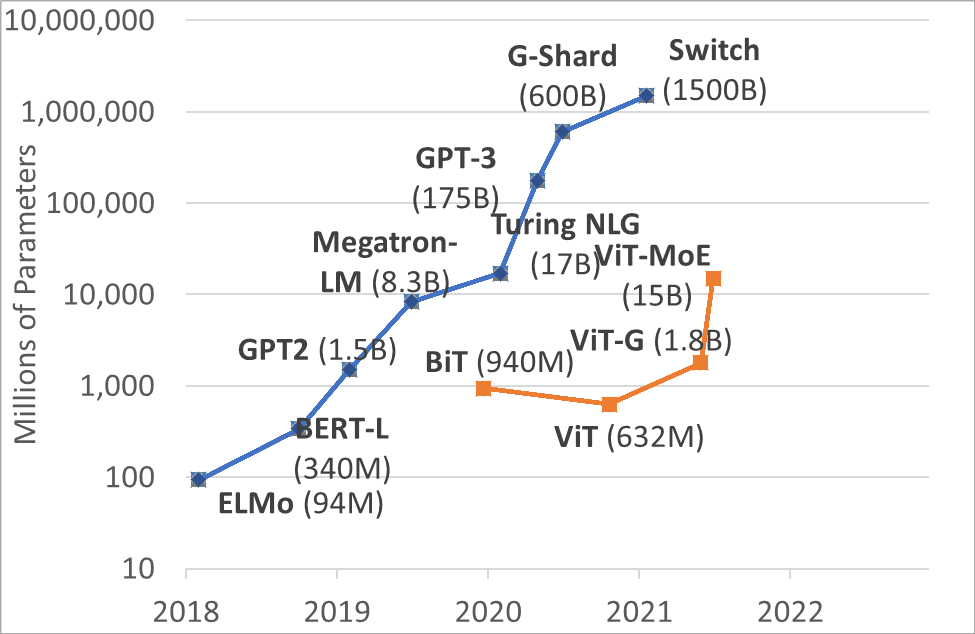
\includegraphics[width=8cm, height=5.5cm]{images/scaling.png}
\centering
\caption{The size records of Vision Transformer in recent years. Retrieved from paperswithcode.com}
\label{fig:scaling}
\end{figure}
\end{enumerate}

\section{Pruning Vision Transformer}

Pruning a deep learning model is a technique to reduce the number of its parameters in order to reduce storage, memory, battery, and hardware consumption without sacrificing its performance. This would allow us to deploy the model and guarantee that it would run smoothly on every device. This section would discuss several techniques to prune a Vision Transformer.

The easiest way to prune a deep learning model is to set a minimum threshold of weight at the end of a layer and any values that is smaller than that threshold will be change to zero. However this method would greatly decrease the performance of the model.

The first comprehensive method to prune a Vision Transformer is to learn its associated importance score before pruning its parameters \cite{pruning-vit}.For the features $x \in \mathbb{R}^{n \times d}$ , where $n$ is the number of features that we want to prune and $d$ is the dimension of each feature, the proposed method will preserve the generated important features and remove the useless ones. Suppose the optimal importance score is $a^* \in \mathbb{R}^d$. Thid method is applied on DeiT-base \cite{deit} trained on ImageNet-1k and ImageNet 100. They managed to reduce the number of parameters by 66.4\% while maintaining the same accuracy with the unpruned model. 

The second pruning method reviewed is block pruning \cite{pruning-block}. They found out that pruning individual parameter is a very hard task for Transformer. They proposed to partition each matrix in the Transformer into multpple fixed-sized blocks. Every acts as an individual group in the regularization with a shared score parameter and a different mask would be applied to each block. This method has not been used alongside a Vision Transformer but they did use it to train BERT \cite{bert}, an encoder-only Transformer language model with 110M parameters for question answering and sentence classification. Overall, they managed to reduce the number of parameters by a factor of 0.25 and increase the training with only a 2\% drop in F1 score.
